

\chapter*{Guía de estilo para escribir un TFG/TFM} \addcontentsline{toc}{chapter}{Guía de estilo}

Este capítulo no forma parte del TFG/TFM. Su único objetivo es aportar algunas recomendaciones y plantillas para tener claro cómo redactar el TFG/TFM. Una vez se haya comprendido, se puede comentar la siguiente línea en el fichero proyecto.tex añadiéndole al principio el carácter \%: 
\begin{verbatim}


\chapter*{Guía de estilo para escribir un TFG/TFM} \addcontentsline{toc}{chapter}{Guía de estilo}

Este capítulo no forma parte del TFG/TFM. Su único objetivo es aportar algunas recomendaciones y plantillas para tener claro cómo redactar el TFG/TFM. Una vez se haya comprendido, se puede comentar la siguiente línea en el fichero proyecto.tex añadiéndole al principio el carácter \%: 
\begin{verbatim}


\chapter*{Guía de estilo para escribir un TFG/TFM} \addcontentsline{toc}{chapter}{Guía de estilo}

Este capítulo no forma parte del TFG/TFM. Su único objetivo es aportar algunas recomendaciones y plantillas para tener claro cómo redactar el TFG/TFM. Una vez se haya comprendido, se puede comentar la siguiente línea en el fichero proyecto.tex añadiéndole al principio el carácter \%: 
\begin{verbatim}


\chapter*{Guía de estilo para escribir un TFG/TFM} \addcontentsline{toc}{chapter}{Guía de estilo}

Este capítulo no forma parte del TFG/TFM. Su único objetivo es aportar algunas recomendaciones y plantillas para tener claro cómo redactar el TFG/TFM. Una vez se haya comprendido, se puede comentar la siguiente línea en el fichero proyecto.tex añadiéndole al principio el carácter \%: 
\begin{verbatim}
\input{guiaDeEstilo} --> %\input{guiaDeEstilo}
\end{verbatim}

\section*{Recomendaciones generales}
A la hora de escribir el TFG/TFM es importante seguir las siguientes recomendaciones: 

\begin{enumerate}
	\item La memoria debe realizarse con el \textbf{máximo cuidado}, y debe proporcionar de forma consistente -y por sí misma- una idea clara y concisa de lo que se ha realizado. 
	\item No debe tener errores tipográficos ni ortográficos. Este es un aspecto que penaliza muchísimo el trabajo en la evaluación del tribunal. 
	\item Siempre que se utilice alguna figura no elaborada por el autor del proyecto debe indicarse la fuente de la que se ha sacado mediante una cita en la bibliografía. 
	\item La lectura debe ser fluida. Por ello, dada la dificultad que tiene afrontar la escritura de un texto largo casi por primera vez, se recomienda elaborar un índice rellenando los títulos de los diferentes apartados de que constará este documento. En segundo lugar, para cada apartado, se indicarán a modo de resumen las diferentes ideas que se desarrollarán posteriormente (una línea de texto por idea). Después, se desarrollan las ideas (cada idea en un párrafo). Cuando se termina, se realiza una lectura completa y detallada del texto para comprobar que es coherente y no tiene fallos ortográficos, tipográficos ni gramaticales, antes de pasarlo al tutor. 
	\item Una extensión normal está entorno a las 100-120 páginas. Esto no quiere decir que tengamos que escribir por escribir, ni meter contenido adicional sin sentido. Hay que escribir el proyecto de forma coherente, pero sin ser telegráfico, esto es, realizando una descripción detallada del trabajo realizado. 
	\item Evitar afirmaciones del tipo “El sistema diseñado es bastante bueno”. Esa misma frase debería ser escrita tal que responda a las preguntas: ¿Qué parte del sistema? ¿En qué sentido? ¿Cuánto de bueno? ¿Comparado con qué?
	\item Evitar la primera persona (incluso del plural). No obstante para resaltar la autoría de algo o enfatizar una posición personal sí se puede usar.
	\item Numerar estructuradamente los capítulos, secciones y subsecciones. Evitar más de tres niveles de anidamiento. 
	\item Toda afirmación categórica o se demuestra (teórica o experimentalmente)  o se incluye una referencia en la que se haya previamente demostrado.
	\item Toda tecnología, teorema, institución, norma, documento que se mencione debe estar referenciado. No incluir referencias a la wiki.
	\item Los términos en ingles que no tenga sentido traducir se pondrán en cursiva al menos para indicar que es un término no castellano.
	 

\end{enumerate}

\section*{Recomendaciones específicas para determinados contenidos}

\subsection*{Inserción de figuras}
Esta es una plantilla de código para adjuntar una figura. 

% El verbatim es solo para poner en el PDF el código que corresponde a la inserción de la figura
\begin{verbatim}
\begin{figure}[t]
	\centering
		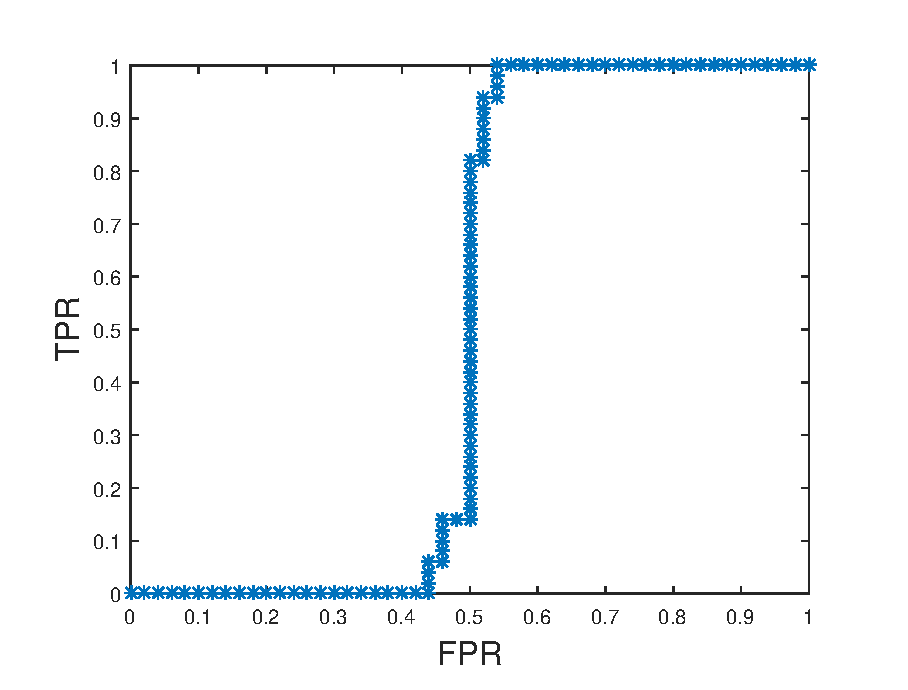
\includegraphics[width=0.6\textwidth]{figuras/prueba.eps}
	\caption{Pie de figura. Poner aquí cita del lugar de donde 
	se ha tomado la imagen en caso de que sea así. }
	\label{fig:prueba}
\end{figure}
\end{verbatim}

% Y ahora pongo la plantilla para que se incluya la figura efectivamente
\begin{figure}[t]
	\centering
	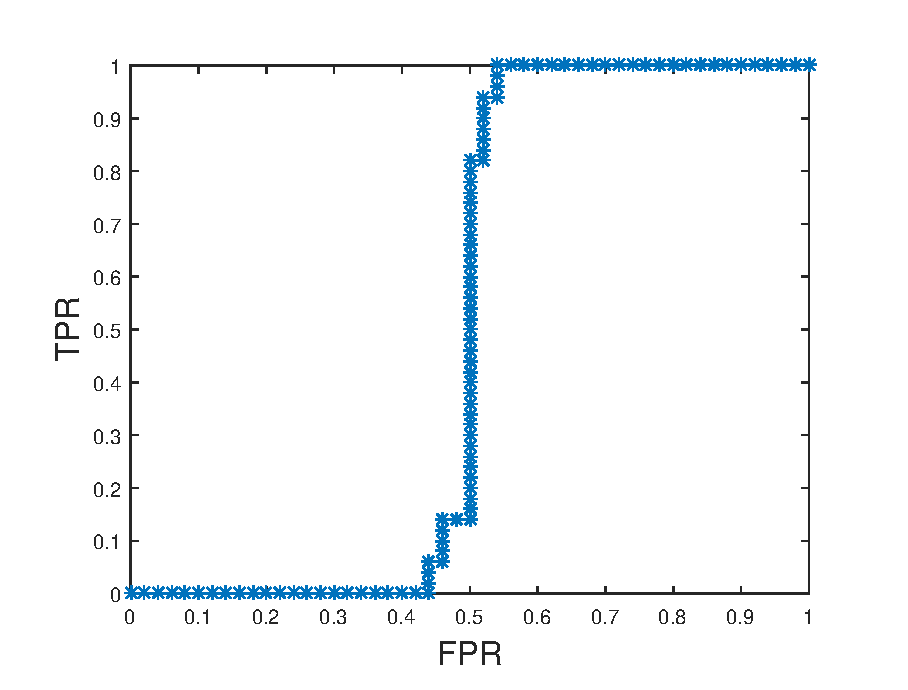
\includegraphics[width=0.6\textwidth]{figuras/prueba.eps}
	\caption{Pie de figura. Poner aquí cita del lugar de donde se ha tomado la imagen en caso de que sea así. }
	\label{fig:prueba}
\end{figure}

Si se pone el modificador [t] (top) latex ubicará la figura en la parte de arriba de la página. Ver otros modificadores como [h] (here) o [b] (bottom). Se pueden usar otras plantillas para, por ejemplo, poner dos figuras una al lado de otra. Consultar en Internet diferentes plantillas en caso de necesidad. 

Cuando en el texto nos refiramos a la figura en cuestión por el número, debemos usar la mayúscula y utilizar referencia a la figura. Esto hará que no nos tengamos que preocupar de la numeración de las figuras. Ej. Como se puede comprobar en la Figura~\ref{fig:prueba}.

Sustituir expresiones del tipo: “En la siguiente figura…” por “En la Figura 2.2…”


\subsection*{Inserción de tablas}

Este sería un ejemplo de una tabla. Se puede modificar el formato y contenido (ver en Internet algún enlace sobre cómo formatear tablas en latex). 

\begin{table}[t]
	\caption{Descripción de la tabla.}
	\label{table:prueba}
	\centering
	\begin{tabular}{l  c} 
		\hline \\[-1.5ex]
		\textbf{Tipo de ataque} & \textbf{Etiqueta} \\ [1ex] 
		\hline\hline \\[-1.5ex]
		DoS11 & dos \\ [0.5ex]
		Exf1MBp & exf1KB \\ [1ex]
		\hline
	\end{tabular}
\end{table}

La forma de referirse a las tablas es similar a las de las figuras (usar mayúsculas y referencia a la etiqueta(label) de la tabla). Ej. Como se puede ver en la Tabla~\ref{table:prueba}, ...


\subsection*{Citas de bibliografía}
Ejemplo de cita de bibliografía. Primero se va a google.scholar y se busca la referencia. Después se da al enlace citar, y se elige el formato bibtex. Se copia ese texto en el fichero bibliografia.bib. Un ejemplo de referenciar una cita es \cite{macia2008evaluation}.


\subsection*{Referencias a secciones}

Para referirnos a secciones, primero debemos tener una etiqueta de tipo \texttt{label} en dicha sección. Posteriormente, pondremos una referencia a dicho label, igual que hacemos para las figuras y las tablas. Ej. Como se ha mencionado en la Sección~\ref{sec:intro:motivacion} (Nótese que la palabra Sección va con mayúscula).

\subsection*{Glosario y acrónimos}

Cuando se utilice un acrónimo se debe definir en el fichero glosario/entradas\_glosario, tal y como está el ejemplo en dicho fichero. Al referirse en el texto se indicará así: \gls{svm} (ver que la primera vez lo pondrá completo). La segunda vez que se referencie a \gls{svm} ya no aparece completo. También se puede nombrar en plural así: \glspl{svm}. 
Otros ejemplos de acrónimo son: \gls{gcd}, \gls{lcm}, \gls{gmf}. 

A la hora de compilar con el glosario, se debe abrir una terminal CMD en el directorio de los fuentes latex del proyecto, y ejecutar el siguiente comando: \texttt{makeglossaries proyecto}. Esto generará los ficheros auxiliares que contienen el glosario. 

\subsection*{Listados de código}

Aquí se puede ver un ejemplo de listado de código: 

%\begin{lstlisting}[frame=none, numbers=none]


\begin{lstlisting}[language=Python,caption=Ejemplo de Python, label=listado:pythonPrueba]
import numpy as np

def incmatrix(genl1,genl2):
	m = len(genl1)
	n = len(genl2)
	M = None #to become the incidence matrix
	VT = np.zeros((n*m,1), int)  #dummy variable

	#compute the bitwise xor matrix
	M1 = bitxormatrix(genl1)
	M2 = np.triu(bitxormatrix(genl2),1) 
	
	for i in range(m-1):
		for j in range(i+1, m):
			[r,c] = np.where(M2 == M1[i,j])
			for k in range(len(r)):
				VT[(i)*n + r[k]] = 1;
				VT[(i)*n + c[k]] = 1;
				VT[(j)*n + r[k]] = 1;
				VT[(j)*n + c[k]] = 1;
	
	if M is None:
		M = np.copy(VT)
	else:
		M = np.concatenate((M, VT), 1)
	
	VT = np.zeros((n*m,1), int)
	
	return M

\end{lstlisting}

Nos podemos referir a él como Listado de código~\ref{listado:pythonPrueba}. 
Si queremos que aparezca como un flotante en la página debemos poner la palabra \texttt{float} así: 
\begin{verbatim}
\begin{lstlisting}[float,language=Python,caption=Ejemplo de Python, 
label=listado:pythonPrueba]
\end{verbatim}


\subsection*{Enlaces URL}
Podemos poner un enlace así \url{http://dtstc.ugr.es/~gmacia} --> %

\chapter*{Guía de estilo para escribir un TFG/TFM} \addcontentsline{toc}{chapter}{Guía de estilo}

Este capítulo no forma parte del TFG/TFM. Su único objetivo es aportar algunas recomendaciones y plantillas para tener claro cómo redactar el TFG/TFM. Una vez se haya comprendido, se puede comentar la siguiente línea en el fichero proyecto.tex añadiéndole al principio el carácter \%: 
\begin{verbatim}
\input{guiaDeEstilo} --> %\input{guiaDeEstilo}
\end{verbatim}

\section*{Recomendaciones generales}
A la hora de escribir el TFG/TFM es importante seguir las siguientes recomendaciones: 

\begin{enumerate}
	\item La memoria debe realizarse con el \textbf{máximo cuidado}, y debe proporcionar de forma consistente -y por sí misma- una idea clara y concisa de lo que se ha realizado. 
	\item No debe tener errores tipográficos ni ortográficos. Este es un aspecto que penaliza muchísimo el trabajo en la evaluación del tribunal. 
	\item Siempre que se utilice alguna figura no elaborada por el autor del proyecto debe indicarse la fuente de la que se ha sacado mediante una cita en la bibliografía. 
	\item La lectura debe ser fluida. Por ello, dada la dificultad que tiene afrontar la escritura de un texto largo casi por primera vez, se recomienda elaborar un índice rellenando los títulos de los diferentes apartados de que constará este documento. En segundo lugar, para cada apartado, se indicarán a modo de resumen las diferentes ideas que se desarrollarán posteriormente (una línea de texto por idea). Después, se desarrollan las ideas (cada idea en un párrafo). Cuando se termina, se realiza una lectura completa y detallada del texto para comprobar que es coherente y no tiene fallos ortográficos, tipográficos ni gramaticales, antes de pasarlo al tutor. 
	\item Una extensión normal está entorno a las 100-120 páginas. Esto no quiere decir que tengamos que escribir por escribir, ni meter contenido adicional sin sentido. Hay que escribir el proyecto de forma coherente, pero sin ser telegráfico, esto es, realizando una descripción detallada del trabajo realizado. 
	\item Evitar afirmaciones del tipo “El sistema diseñado es bastante bueno”. Esa misma frase debería ser escrita tal que responda a las preguntas: ¿Qué parte del sistema? ¿En qué sentido? ¿Cuánto de bueno? ¿Comparado con qué?
	\item Evitar la primera persona (incluso del plural). No obstante para resaltar la autoría de algo o enfatizar una posición personal sí se puede usar.
	\item Numerar estructuradamente los capítulos, secciones y subsecciones. Evitar más de tres niveles de anidamiento. 
	\item Toda afirmación categórica o se demuestra (teórica o experimentalmente)  o se incluye una referencia en la que se haya previamente demostrado.
	\item Toda tecnología, teorema, institución, norma, documento que se mencione debe estar referenciado. No incluir referencias a la wiki.
	\item Los términos en ingles que no tenga sentido traducir se pondrán en cursiva al menos para indicar que es un término no castellano.
	 

\end{enumerate}

\section*{Recomendaciones específicas para determinados contenidos}

\subsection*{Inserción de figuras}
Esta es una plantilla de código para adjuntar una figura. 

% El verbatim es solo para poner en el PDF el código que corresponde a la inserción de la figura
\begin{verbatim}
\begin{figure}[t]
	\centering
		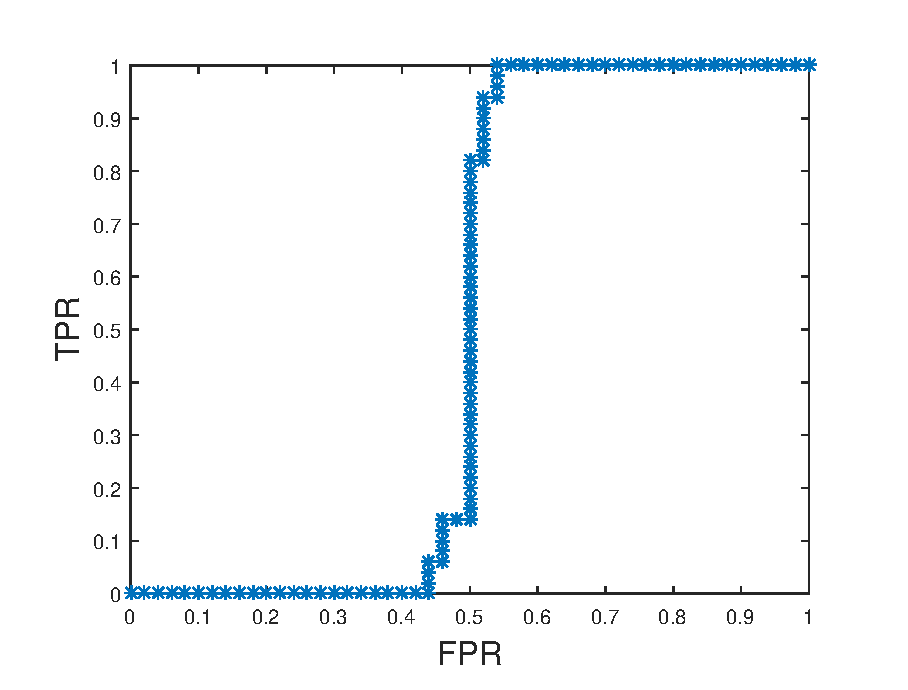
\includegraphics[width=0.6\textwidth]{figuras/prueba.eps}
	\caption{Pie de figura. Poner aquí cita del lugar de donde 
	se ha tomado la imagen en caso de que sea así. }
	\label{fig:prueba}
\end{figure}
\end{verbatim}

% Y ahora pongo la plantilla para que se incluya la figura efectivamente
\begin{figure}[t]
	\centering
	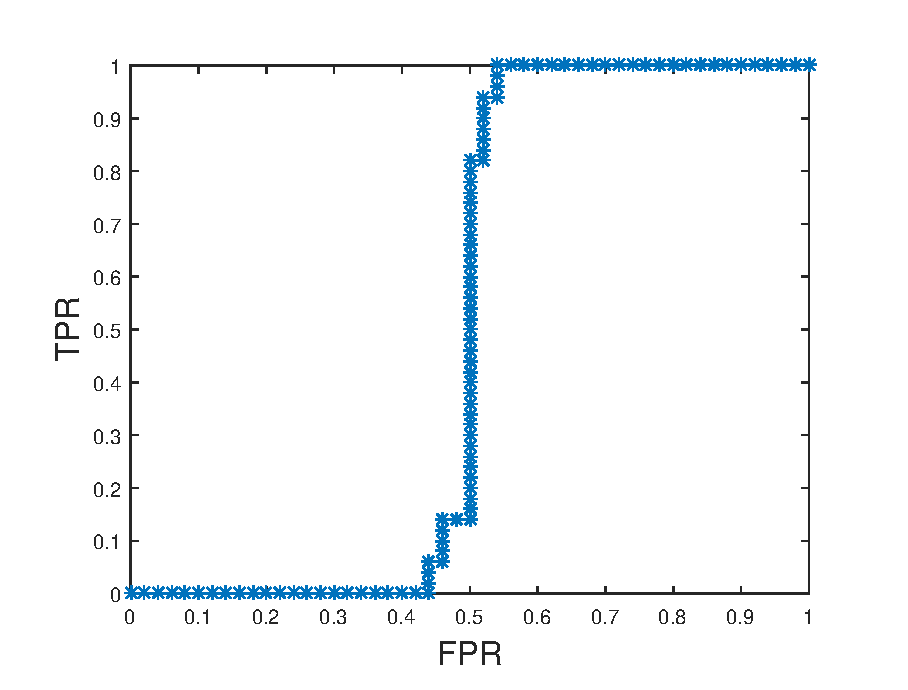
\includegraphics[width=0.6\textwidth]{figuras/prueba.eps}
	\caption{Pie de figura. Poner aquí cita del lugar de donde se ha tomado la imagen en caso de que sea así. }
	\label{fig:prueba}
\end{figure}

Si se pone el modificador [t] (top) latex ubicará la figura en la parte de arriba de la página. Ver otros modificadores como [h] (here) o [b] (bottom). Se pueden usar otras plantillas para, por ejemplo, poner dos figuras una al lado de otra. Consultar en Internet diferentes plantillas en caso de necesidad. 

Cuando en el texto nos refiramos a la figura en cuestión por el número, debemos usar la mayúscula y utilizar referencia a la figura. Esto hará que no nos tengamos que preocupar de la numeración de las figuras. Ej. Como se puede comprobar en la Figura~\ref{fig:prueba}.

Sustituir expresiones del tipo: “En la siguiente figura…” por “En la Figura 2.2…”


\subsection*{Inserción de tablas}

Este sería un ejemplo de una tabla. Se puede modificar el formato y contenido (ver en Internet algún enlace sobre cómo formatear tablas en latex). 

\begin{table}[t]
	\caption{Descripción de la tabla.}
	\label{table:prueba}
	\centering
	\begin{tabular}{l  c} 
		\hline \\[-1.5ex]
		\textbf{Tipo de ataque} & \textbf{Etiqueta} \\ [1ex] 
		\hline\hline \\[-1.5ex]
		DoS11 & dos \\ [0.5ex]
		Exf1MBp & exf1KB \\ [1ex]
		\hline
	\end{tabular}
\end{table}

La forma de referirse a las tablas es similar a las de las figuras (usar mayúsculas y referencia a la etiqueta(label) de la tabla). Ej. Como se puede ver en la Tabla~\ref{table:prueba}, ...


\subsection*{Citas de bibliografía}
Ejemplo de cita de bibliografía. Primero se va a google.scholar y se busca la referencia. Después se da al enlace citar, y se elige el formato bibtex. Se copia ese texto en el fichero bibliografia.bib. Un ejemplo de referenciar una cita es \cite{macia2008evaluation}.


\subsection*{Referencias a secciones}

Para referirnos a secciones, primero debemos tener una etiqueta de tipo \texttt{label} en dicha sección. Posteriormente, pondremos una referencia a dicho label, igual que hacemos para las figuras y las tablas. Ej. Como se ha mencionado en la Sección~\ref{sec:intro:motivacion} (Nótese que la palabra Sección va con mayúscula).

\subsection*{Glosario y acrónimos}

Cuando se utilice un acrónimo se debe definir en el fichero glosario/entradas\_glosario, tal y como está el ejemplo en dicho fichero. Al referirse en el texto se indicará así: \gls{svm} (ver que la primera vez lo pondrá completo). La segunda vez que se referencie a \gls{svm} ya no aparece completo. También se puede nombrar en plural así: \glspl{svm}. 
Otros ejemplos de acrónimo son: \gls{gcd}, \gls{lcm}, \gls{gmf}. 

A la hora de compilar con el glosario, se debe abrir una terminal CMD en el directorio de los fuentes latex del proyecto, y ejecutar el siguiente comando: \texttt{makeglossaries proyecto}. Esto generará los ficheros auxiliares que contienen el glosario. 

\subsection*{Listados de código}

Aquí se puede ver un ejemplo de listado de código: 

%\begin{lstlisting}[frame=none, numbers=none]


\begin{lstlisting}[language=Python,caption=Ejemplo de Python, label=listado:pythonPrueba]
import numpy as np

def incmatrix(genl1,genl2):
	m = len(genl1)
	n = len(genl2)
	M = None #to become the incidence matrix
	VT = np.zeros((n*m,1), int)  #dummy variable

	#compute the bitwise xor matrix
	M1 = bitxormatrix(genl1)
	M2 = np.triu(bitxormatrix(genl2),1) 
	
	for i in range(m-1):
		for j in range(i+1, m):
			[r,c] = np.where(M2 == M1[i,j])
			for k in range(len(r)):
				VT[(i)*n + r[k]] = 1;
				VT[(i)*n + c[k]] = 1;
				VT[(j)*n + r[k]] = 1;
				VT[(j)*n + c[k]] = 1;
	
	if M is None:
		M = np.copy(VT)
	else:
		M = np.concatenate((M, VT), 1)
	
	VT = np.zeros((n*m,1), int)
	
	return M

\end{lstlisting}

Nos podemos referir a él como Listado de código~\ref{listado:pythonPrueba}. 
Si queremos que aparezca como un flotante en la página debemos poner la palabra \texttt{float} así: 
\begin{verbatim}
\begin{lstlisting}[float,language=Python,caption=Ejemplo de Python, 
label=listado:pythonPrueba]
\end{verbatim}


\subsection*{Enlaces URL}
Podemos poner un enlace así \url{http://dtstc.ugr.es/~gmacia}
\end{verbatim}

\section*{Recomendaciones generales}
A la hora de escribir el TFG/TFM es importante seguir las siguientes recomendaciones: 

\begin{enumerate}
	\item La memoria debe realizarse con el \textbf{máximo cuidado}, y debe proporcionar de forma consistente -y por sí misma- una idea clara y concisa de lo que se ha realizado. 
	\item No debe tener errores tipográficos ni ortográficos. Este es un aspecto que penaliza muchísimo el trabajo en la evaluación del tribunal. 
	\item Siempre que se utilice alguna figura no elaborada por el autor del proyecto debe indicarse la fuente de la que se ha sacado mediante una cita en la bibliografía. 
	\item La lectura debe ser fluida. Por ello, dada la dificultad que tiene afrontar la escritura de un texto largo casi por primera vez, se recomienda elaborar un índice rellenando los títulos de los diferentes apartados de que constará este documento. En segundo lugar, para cada apartado, se indicarán a modo de resumen las diferentes ideas que se desarrollarán posteriormente (una línea de texto por idea). Después, se desarrollan las ideas (cada idea en un párrafo). Cuando se termina, se realiza una lectura completa y detallada del texto para comprobar que es coherente y no tiene fallos ortográficos, tipográficos ni gramaticales, antes de pasarlo al tutor. 
	\item Una extensión normal está entorno a las 100-120 páginas. Esto no quiere decir que tengamos que escribir por escribir, ni meter contenido adicional sin sentido. Hay que escribir el proyecto de forma coherente, pero sin ser telegráfico, esto es, realizando una descripción detallada del trabajo realizado. 
	\item Evitar afirmaciones del tipo “El sistema diseñado es bastante bueno”. Esa misma frase debería ser escrita tal que responda a las preguntas: ¿Qué parte del sistema? ¿En qué sentido? ¿Cuánto de bueno? ¿Comparado con qué?
	\item Evitar la primera persona (incluso del plural). No obstante para resaltar la autoría de algo o enfatizar una posición personal sí se puede usar.
	\item Numerar estructuradamente los capítulos, secciones y subsecciones. Evitar más de tres niveles de anidamiento. 
	\item Toda afirmación categórica o se demuestra (teórica o experimentalmente)  o se incluye una referencia en la que se haya previamente demostrado.
	\item Toda tecnología, teorema, institución, norma, documento que se mencione debe estar referenciado. No incluir referencias a la wiki.
	\item Los términos en ingles que no tenga sentido traducir se pondrán en cursiva al menos para indicar que es un término no castellano.
	 

\end{enumerate}

\section*{Recomendaciones específicas para determinados contenidos}

\subsection*{Inserción de figuras}
Esta es una plantilla de código para adjuntar una figura. 

% El verbatim es solo para poner en el PDF el código que corresponde a la inserción de la figura
\begin{verbatim}
\begin{figure}[t]
	\centering
		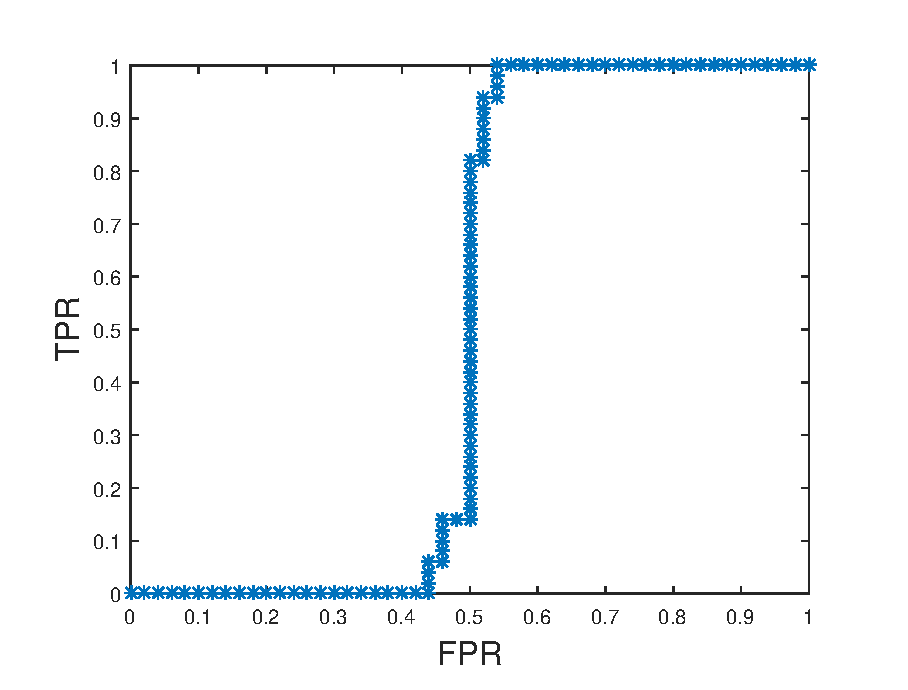
\includegraphics[width=0.6\textwidth]{figuras/prueba.eps}
	\caption{Pie de figura. Poner aquí cita del lugar de donde 
	se ha tomado la imagen en caso de que sea así. }
	\label{fig:prueba}
\end{figure}
\end{verbatim}

% Y ahora pongo la plantilla para que se incluya la figura efectivamente
\begin{figure}[t]
	\centering
	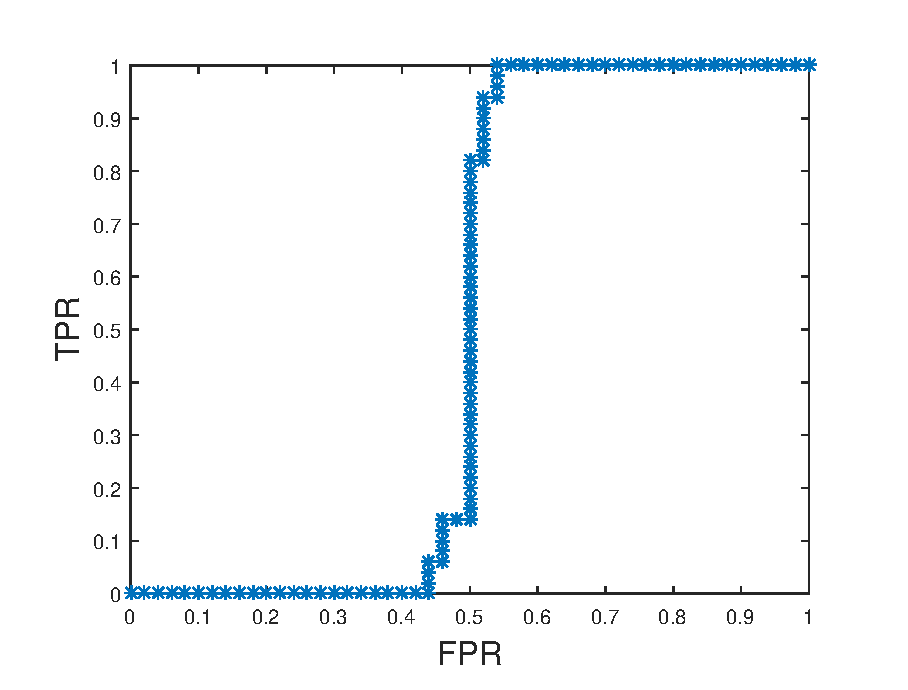
\includegraphics[width=0.6\textwidth]{figuras/prueba.eps}
	\caption{Pie de figura. Poner aquí cita del lugar de donde se ha tomado la imagen en caso de que sea así. }
	\label{fig:prueba}
\end{figure}

Si se pone el modificador [t] (top) latex ubicará la figura en la parte de arriba de la página. Ver otros modificadores como [h] (here) o [b] (bottom). Se pueden usar otras plantillas para, por ejemplo, poner dos figuras una al lado de otra. Consultar en Internet diferentes plantillas en caso de necesidad. 

Cuando en el texto nos refiramos a la figura en cuestión por el número, debemos usar la mayúscula y utilizar referencia a la figura. Esto hará que no nos tengamos que preocupar de la numeración de las figuras. Ej. Como se puede comprobar en la Figura~\ref{fig:prueba}.

Sustituir expresiones del tipo: “En la siguiente figura…” por “En la Figura 2.2…”


\subsection*{Inserción de tablas}

Este sería un ejemplo de una tabla. Se puede modificar el formato y contenido (ver en Internet algún enlace sobre cómo formatear tablas en latex). 

\begin{table}[t]
	\caption{Descripción de la tabla.}
	\label{table:prueba}
	\centering
	\begin{tabular}{l  c} 
		\hline \\[-1.5ex]
		\textbf{Tipo de ataque} & \textbf{Etiqueta} \\ [1ex] 
		\hline\hline \\[-1.5ex]
		DoS11 & dos \\ [0.5ex]
		Exf1MBp & exf1KB \\ [1ex]
		\hline
	\end{tabular}
\end{table}

La forma de referirse a las tablas es similar a las de las figuras (usar mayúsculas y referencia a la etiqueta(label) de la tabla). Ej. Como se puede ver en la Tabla~\ref{table:prueba}, ...


\subsection*{Citas de bibliografía}
Ejemplo de cita de bibliografía. Primero se va a google.scholar y se busca la referencia. Después se da al enlace citar, y se elige el formato bibtex. Se copia ese texto en el fichero bibliografia.bib. Un ejemplo de referenciar una cita es \cite{macia2008evaluation}.


\subsection*{Referencias a secciones}

Para referirnos a secciones, primero debemos tener una etiqueta de tipo \texttt{label} en dicha sección. Posteriormente, pondremos una referencia a dicho label, igual que hacemos para las figuras y las tablas. Ej. Como se ha mencionado en la Sección~\ref{sec:intro:motivacion} (Nótese que la palabra Sección va con mayúscula).

\subsection*{Glosario y acrónimos}

Cuando se utilice un acrónimo se debe definir en el fichero glosario/entradas\_glosario, tal y como está el ejemplo en dicho fichero. Al referirse en el texto se indicará así: \gls{svm} (ver que la primera vez lo pondrá completo). La segunda vez que se referencie a \gls{svm} ya no aparece completo. También se puede nombrar en plural así: \glspl{svm}. 
Otros ejemplos de acrónimo son: \gls{gcd}, \gls{lcm}, \gls{gmf}. 

A la hora de compilar con el glosario, se debe abrir una terminal CMD en el directorio de los fuentes latex del proyecto, y ejecutar el siguiente comando: \texttt{makeglossaries proyecto}. Esto generará los ficheros auxiliares que contienen el glosario. 

\subsection*{Listados de código}

Aquí se puede ver un ejemplo de listado de código: 

%\begin{lstlisting}[frame=none, numbers=none]


\begin{lstlisting}[language=Python,caption=Ejemplo de Python, label=listado:pythonPrueba]
import numpy as np

def incmatrix(genl1,genl2):
	m = len(genl1)
	n = len(genl2)
	M = None #to become the incidence matrix
	VT = np.zeros((n*m,1), int)  #dummy variable

	#compute the bitwise xor matrix
	M1 = bitxormatrix(genl1)
	M2 = np.triu(bitxormatrix(genl2),1) 
	
	for i in range(m-1):
		for j in range(i+1, m):
			[r,c] = np.where(M2 == M1[i,j])
			for k in range(len(r)):
				VT[(i)*n + r[k]] = 1;
				VT[(i)*n + c[k]] = 1;
				VT[(j)*n + r[k]] = 1;
				VT[(j)*n + c[k]] = 1;
	
	if M is None:
		M = np.copy(VT)
	else:
		M = np.concatenate((M, VT), 1)
	
	VT = np.zeros((n*m,1), int)
	
	return M

\end{lstlisting}

Nos podemos referir a él como Listado de código~\ref{listado:pythonPrueba}. 
Si queremos que aparezca como un flotante en la página debemos poner la palabra \texttt{float} así: 
\begin{verbatim}
\begin{lstlisting}[float,language=Python,caption=Ejemplo de Python, 
label=listado:pythonPrueba]
\end{verbatim}


\subsection*{Enlaces URL}
Podemos poner un enlace así \url{http://dtstc.ugr.es/~gmacia} --> %

\chapter*{Guía de estilo para escribir un TFG/TFM} \addcontentsline{toc}{chapter}{Guía de estilo}

Este capítulo no forma parte del TFG/TFM. Su único objetivo es aportar algunas recomendaciones y plantillas para tener claro cómo redactar el TFG/TFM. Una vez se haya comprendido, se puede comentar la siguiente línea en el fichero proyecto.tex añadiéndole al principio el carácter \%: 
\begin{verbatim}


\chapter*{Guía de estilo para escribir un TFG/TFM} \addcontentsline{toc}{chapter}{Guía de estilo}

Este capítulo no forma parte del TFG/TFM. Su único objetivo es aportar algunas recomendaciones y plantillas para tener claro cómo redactar el TFG/TFM. Una vez se haya comprendido, se puede comentar la siguiente línea en el fichero proyecto.tex añadiéndole al principio el carácter \%: 
\begin{verbatim}
\input{guiaDeEstilo} --> %\input{guiaDeEstilo}
\end{verbatim}

\section*{Recomendaciones generales}
A la hora de escribir el TFG/TFM es importante seguir las siguientes recomendaciones: 

\begin{enumerate}
	\item La memoria debe realizarse con el \textbf{máximo cuidado}, y debe proporcionar de forma consistente -y por sí misma- una idea clara y concisa de lo que se ha realizado. 
	\item No debe tener errores tipográficos ni ortográficos. Este es un aspecto que penaliza muchísimo el trabajo en la evaluación del tribunal. 
	\item Siempre que se utilice alguna figura no elaborada por el autor del proyecto debe indicarse la fuente de la que se ha sacado mediante una cita en la bibliografía. 
	\item La lectura debe ser fluida. Por ello, dada la dificultad que tiene afrontar la escritura de un texto largo casi por primera vez, se recomienda elaborar un índice rellenando los títulos de los diferentes apartados de que constará este documento. En segundo lugar, para cada apartado, se indicarán a modo de resumen las diferentes ideas que se desarrollarán posteriormente (una línea de texto por idea). Después, se desarrollan las ideas (cada idea en un párrafo). Cuando se termina, se realiza una lectura completa y detallada del texto para comprobar que es coherente y no tiene fallos ortográficos, tipográficos ni gramaticales, antes de pasarlo al tutor. 
	\item Una extensión normal está entorno a las 100-120 páginas. Esto no quiere decir que tengamos que escribir por escribir, ni meter contenido adicional sin sentido. Hay que escribir el proyecto de forma coherente, pero sin ser telegráfico, esto es, realizando una descripción detallada del trabajo realizado. 
	\item Evitar afirmaciones del tipo “El sistema diseñado es bastante bueno”. Esa misma frase debería ser escrita tal que responda a las preguntas: ¿Qué parte del sistema? ¿En qué sentido? ¿Cuánto de bueno? ¿Comparado con qué?
	\item Evitar la primera persona (incluso del plural). No obstante para resaltar la autoría de algo o enfatizar una posición personal sí se puede usar.
	\item Numerar estructuradamente los capítulos, secciones y subsecciones. Evitar más de tres niveles de anidamiento. 
	\item Toda afirmación categórica o se demuestra (teórica o experimentalmente)  o se incluye una referencia en la que se haya previamente demostrado.
	\item Toda tecnología, teorema, institución, norma, documento que se mencione debe estar referenciado. No incluir referencias a la wiki.
	\item Los términos en ingles que no tenga sentido traducir se pondrán en cursiva al menos para indicar que es un término no castellano.
	 

\end{enumerate}

\section*{Recomendaciones específicas para determinados contenidos}

\subsection*{Inserción de figuras}
Esta es una plantilla de código para adjuntar una figura. 

% El verbatim es solo para poner en el PDF el código que corresponde a la inserción de la figura
\begin{verbatim}
\begin{figure}[t]
	\centering
		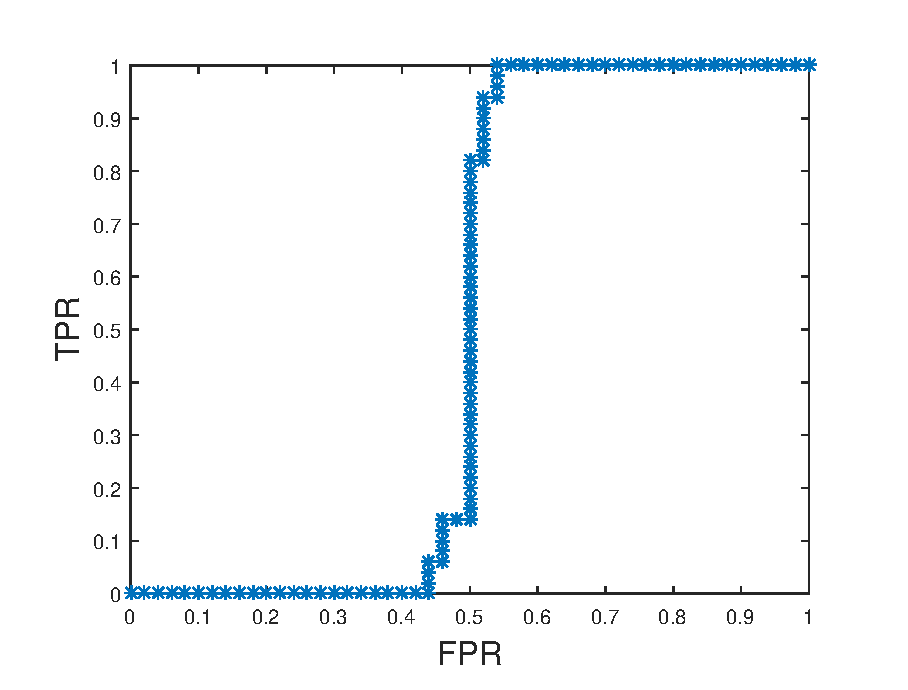
\includegraphics[width=0.6\textwidth]{figuras/prueba.eps}
	\caption{Pie de figura. Poner aquí cita del lugar de donde 
	se ha tomado la imagen en caso de que sea así. }
	\label{fig:prueba}
\end{figure}
\end{verbatim}

% Y ahora pongo la plantilla para que se incluya la figura efectivamente
\begin{figure}[t]
	\centering
	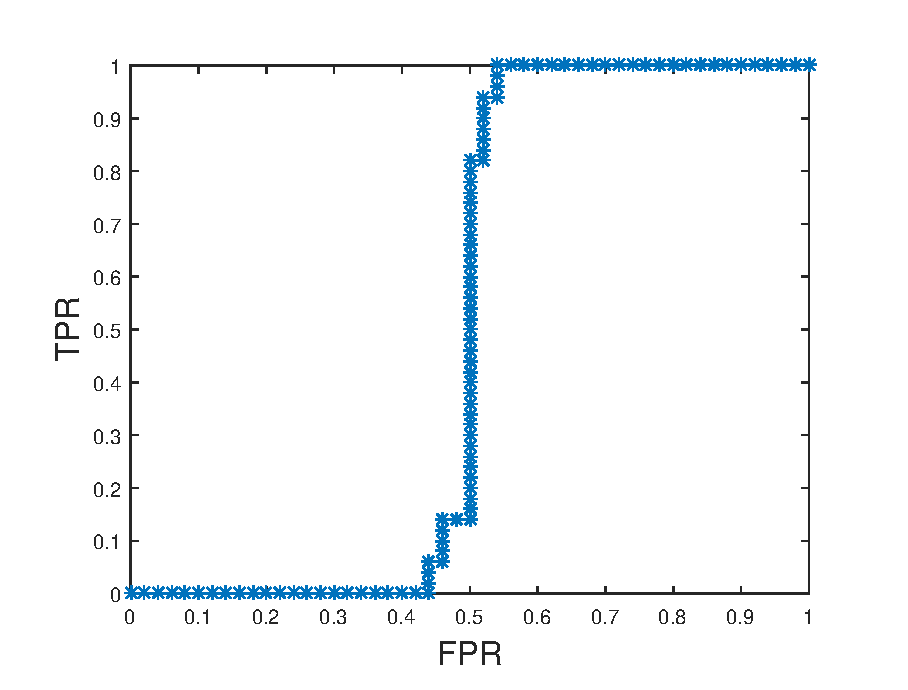
\includegraphics[width=0.6\textwidth]{figuras/prueba.eps}
	\caption{Pie de figura. Poner aquí cita del lugar de donde se ha tomado la imagen en caso de que sea así. }
	\label{fig:prueba}
\end{figure}

Si se pone el modificador [t] (top) latex ubicará la figura en la parte de arriba de la página. Ver otros modificadores como [h] (here) o [b] (bottom). Se pueden usar otras plantillas para, por ejemplo, poner dos figuras una al lado de otra. Consultar en Internet diferentes plantillas en caso de necesidad. 

Cuando en el texto nos refiramos a la figura en cuestión por el número, debemos usar la mayúscula y utilizar referencia a la figura. Esto hará que no nos tengamos que preocupar de la numeración de las figuras. Ej. Como se puede comprobar en la Figura~\ref{fig:prueba}.

Sustituir expresiones del tipo: “En la siguiente figura…” por “En la Figura 2.2…”


\subsection*{Inserción de tablas}

Este sería un ejemplo de una tabla. Se puede modificar el formato y contenido (ver en Internet algún enlace sobre cómo formatear tablas en latex). 

\begin{table}[t]
	\caption{Descripción de la tabla.}
	\label{table:prueba}
	\centering
	\begin{tabular}{l  c} 
		\hline \\[-1.5ex]
		\textbf{Tipo de ataque} & \textbf{Etiqueta} \\ [1ex] 
		\hline\hline \\[-1.5ex]
		DoS11 & dos \\ [0.5ex]
		Exf1MBp & exf1KB \\ [1ex]
		\hline
	\end{tabular}
\end{table}

La forma de referirse a las tablas es similar a las de las figuras (usar mayúsculas y referencia a la etiqueta(label) de la tabla). Ej. Como se puede ver en la Tabla~\ref{table:prueba}, ...


\subsection*{Citas de bibliografía}
Ejemplo de cita de bibliografía. Primero se va a google.scholar y se busca la referencia. Después se da al enlace citar, y se elige el formato bibtex. Se copia ese texto en el fichero bibliografia.bib. Un ejemplo de referenciar una cita es \cite{macia2008evaluation}.


\subsection*{Referencias a secciones}

Para referirnos a secciones, primero debemos tener una etiqueta de tipo \texttt{label} en dicha sección. Posteriormente, pondremos una referencia a dicho label, igual que hacemos para las figuras y las tablas. Ej. Como se ha mencionado en la Sección~\ref{sec:intro:motivacion} (Nótese que la palabra Sección va con mayúscula).

\subsection*{Glosario y acrónimos}

Cuando se utilice un acrónimo se debe definir en el fichero glosario/entradas\_glosario, tal y como está el ejemplo en dicho fichero. Al referirse en el texto se indicará así: \gls{svm} (ver que la primera vez lo pondrá completo). La segunda vez que se referencie a \gls{svm} ya no aparece completo. También se puede nombrar en plural así: \glspl{svm}. 
Otros ejemplos de acrónimo son: \gls{gcd}, \gls{lcm}, \gls{gmf}. 

A la hora de compilar con el glosario, se debe abrir una terminal CMD en el directorio de los fuentes latex del proyecto, y ejecutar el siguiente comando: \texttt{makeglossaries proyecto}. Esto generará los ficheros auxiliares que contienen el glosario. 

\subsection*{Listados de código}

Aquí se puede ver un ejemplo de listado de código: 

%\begin{lstlisting}[frame=none, numbers=none]


\begin{lstlisting}[language=Python,caption=Ejemplo de Python, label=listado:pythonPrueba]
import numpy as np

def incmatrix(genl1,genl2):
	m = len(genl1)
	n = len(genl2)
	M = None #to become the incidence matrix
	VT = np.zeros((n*m,1), int)  #dummy variable

	#compute the bitwise xor matrix
	M1 = bitxormatrix(genl1)
	M2 = np.triu(bitxormatrix(genl2),1) 
	
	for i in range(m-1):
		for j in range(i+1, m):
			[r,c] = np.where(M2 == M1[i,j])
			for k in range(len(r)):
				VT[(i)*n + r[k]] = 1;
				VT[(i)*n + c[k]] = 1;
				VT[(j)*n + r[k]] = 1;
				VT[(j)*n + c[k]] = 1;
	
	if M is None:
		M = np.copy(VT)
	else:
		M = np.concatenate((M, VT), 1)
	
	VT = np.zeros((n*m,1), int)
	
	return M

\end{lstlisting}

Nos podemos referir a él como Listado de código~\ref{listado:pythonPrueba}. 
Si queremos que aparezca como un flotante en la página debemos poner la palabra \texttt{float} así: 
\begin{verbatim}
\begin{lstlisting}[float,language=Python,caption=Ejemplo de Python, 
label=listado:pythonPrueba]
\end{verbatim}


\subsection*{Enlaces URL}
Podemos poner un enlace así \url{http://dtstc.ugr.es/~gmacia} --> %

\chapter*{Guía de estilo para escribir un TFG/TFM} \addcontentsline{toc}{chapter}{Guía de estilo}

Este capítulo no forma parte del TFG/TFM. Su único objetivo es aportar algunas recomendaciones y plantillas para tener claro cómo redactar el TFG/TFM. Una vez se haya comprendido, se puede comentar la siguiente línea en el fichero proyecto.tex añadiéndole al principio el carácter \%: 
\begin{verbatim}
\input{guiaDeEstilo} --> %\input{guiaDeEstilo}
\end{verbatim}

\section*{Recomendaciones generales}
A la hora de escribir el TFG/TFM es importante seguir las siguientes recomendaciones: 

\begin{enumerate}
	\item La memoria debe realizarse con el \textbf{máximo cuidado}, y debe proporcionar de forma consistente -y por sí misma- una idea clara y concisa de lo que se ha realizado. 
	\item No debe tener errores tipográficos ni ortográficos. Este es un aspecto que penaliza muchísimo el trabajo en la evaluación del tribunal. 
	\item Siempre que se utilice alguna figura no elaborada por el autor del proyecto debe indicarse la fuente de la que se ha sacado mediante una cita en la bibliografía. 
	\item La lectura debe ser fluida. Por ello, dada la dificultad que tiene afrontar la escritura de un texto largo casi por primera vez, se recomienda elaborar un índice rellenando los títulos de los diferentes apartados de que constará este documento. En segundo lugar, para cada apartado, se indicarán a modo de resumen las diferentes ideas que se desarrollarán posteriormente (una línea de texto por idea). Después, se desarrollan las ideas (cada idea en un párrafo). Cuando se termina, se realiza una lectura completa y detallada del texto para comprobar que es coherente y no tiene fallos ortográficos, tipográficos ni gramaticales, antes de pasarlo al tutor. 
	\item Una extensión normal está entorno a las 100-120 páginas. Esto no quiere decir que tengamos que escribir por escribir, ni meter contenido adicional sin sentido. Hay que escribir el proyecto de forma coherente, pero sin ser telegráfico, esto es, realizando una descripción detallada del trabajo realizado. 
	\item Evitar afirmaciones del tipo “El sistema diseñado es bastante bueno”. Esa misma frase debería ser escrita tal que responda a las preguntas: ¿Qué parte del sistema? ¿En qué sentido? ¿Cuánto de bueno? ¿Comparado con qué?
	\item Evitar la primera persona (incluso del plural). No obstante para resaltar la autoría de algo o enfatizar una posición personal sí se puede usar.
	\item Numerar estructuradamente los capítulos, secciones y subsecciones. Evitar más de tres niveles de anidamiento. 
	\item Toda afirmación categórica o se demuestra (teórica o experimentalmente)  o se incluye una referencia en la que se haya previamente demostrado.
	\item Toda tecnología, teorema, institución, norma, documento que se mencione debe estar referenciado. No incluir referencias a la wiki.
	\item Los términos en ingles que no tenga sentido traducir se pondrán en cursiva al menos para indicar que es un término no castellano.
	 

\end{enumerate}

\section*{Recomendaciones específicas para determinados contenidos}

\subsection*{Inserción de figuras}
Esta es una plantilla de código para adjuntar una figura. 

% El verbatim es solo para poner en el PDF el código que corresponde a la inserción de la figura
\begin{verbatim}
\begin{figure}[t]
	\centering
		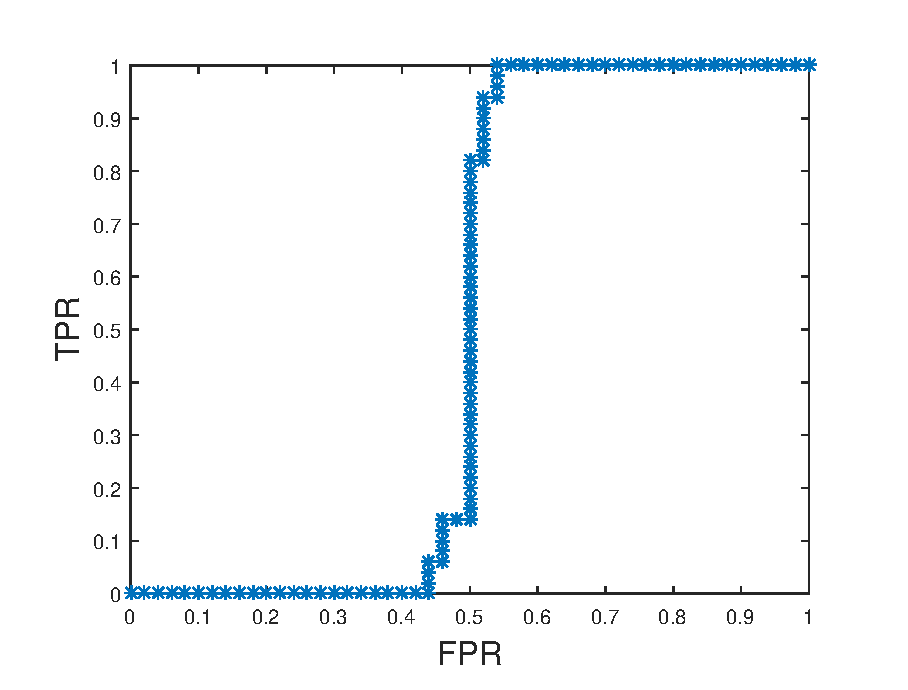
\includegraphics[width=0.6\textwidth]{figuras/prueba.eps}
	\caption{Pie de figura. Poner aquí cita del lugar de donde 
	se ha tomado la imagen en caso de que sea así. }
	\label{fig:prueba}
\end{figure}
\end{verbatim}

% Y ahora pongo la plantilla para que se incluya la figura efectivamente
\begin{figure}[t]
	\centering
	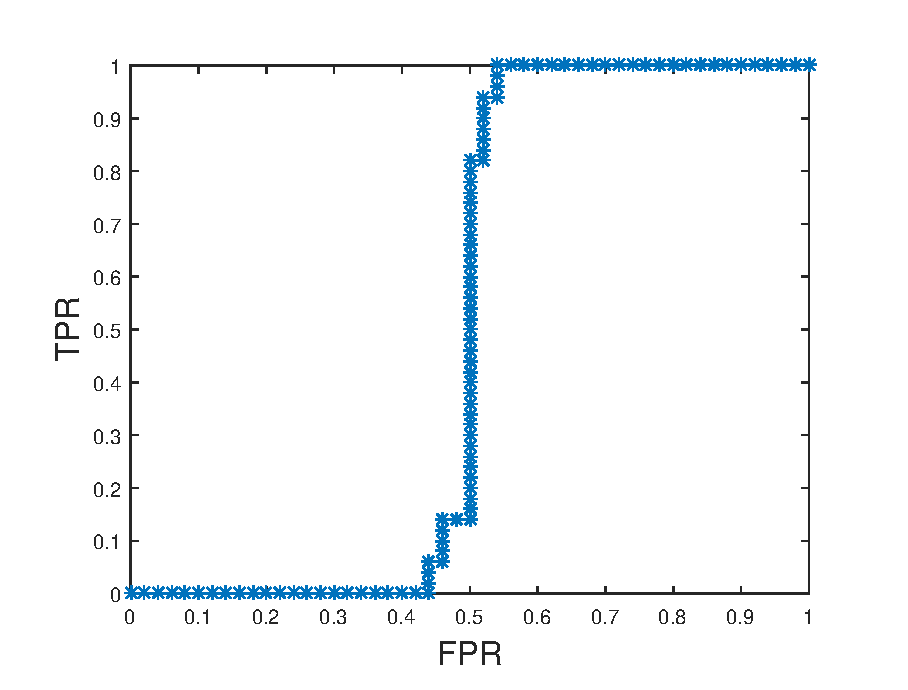
\includegraphics[width=0.6\textwidth]{figuras/prueba.eps}
	\caption{Pie de figura. Poner aquí cita del lugar de donde se ha tomado la imagen en caso de que sea así. }
	\label{fig:prueba}
\end{figure}

Si se pone el modificador [t] (top) latex ubicará la figura en la parte de arriba de la página. Ver otros modificadores como [h] (here) o [b] (bottom). Se pueden usar otras plantillas para, por ejemplo, poner dos figuras una al lado de otra. Consultar en Internet diferentes plantillas en caso de necesidad. 

Cuando en el texto nos refiramos a la figura en cuestión por el número, debemos usar la mayúscula y utilizar referencia a la figura. Esto hará que no nos tengamos que preocupar de la numeración de las figuras. Ej. Como se puede comprobar en la Figura~\ref{fig:prueba}.

Sustituir expresiones del tipo: “En la siguiente figura…” por “En la Figura 2.2…”


\subsection*{Inserción de tablas}

Este sería un ejemplo de una tabla. Se puede modificar el formato y contenido (ver en Internet algún enlace sobre cómo formatear tablas en latex). 

\begin{table}[t]
	\caption{Descripción de la tabla.}
	\label{table:prueba}
	\centering
	\begin{tabular}{l  c} 
		\hline \\[-1.5ex]
		\textbf{Tipo de ataque} & \textbf{Etiqueta} \\ [1ex] 
		\hline\hline \\[-1.5ex]
		DoS11 & dos \\ [0.5ex]
		Exf1MBp & exf1KB \\ [1ex]
		\hline
	\end{tabular}
\end{table}

La forma de referirse a las tablas es similar a las de las figuras (usar mayúsculas y referencia a la etiqueta(label) de la tabla). Ej. Como se puede ver en la Tabla~\ref{table:prueba}, ...


\subsection*{Citas de bibliografía}
Ejemplo de cita de bibliografía. Primero se va a google.scholar y se busca la referencia. Después se da al enlace citar, y se elige el formato bibtex. Se copia ese texto en el fichero bibliografia.bib. Un ejemplo de referenciar una cita es \cite{macia2008evaluation}.


\subsection*{Referencias a secciones}

Para referirnos a secciones, primero debemos tener una etiqueta de tipo \texttt{label} en dicha sección. Posteriormente, pondremos una referencia a dicho label, igual que hacemos para las figuras y las tablas. Ej. Como se ha mencionado en la Sección~\ref{sec:intro:motivacion} (Nótese que la palabra Sección va con mayúscula).

\subsection*{Glosario y acrónimos}

Cuando se utilice un acrónimo se debe definir en el fichero glosario/entradas\_glosario, tal y como está el ejemplo en dicho fichero. Al referirse en el texto se indicará así: \gls{svm} (ver que la primera vez lo pondrá completo). La segunda vez que se referencie a \gls{svm} ya no aparece completo. También se puede nombrar en plural así: \glspl{svm}. 
Otros ejemplos de acrónimo son: \gls{gcd}, \gls{lcm}, \gls{gmf}. 

A la hora de compilar con el glosario, se debe abrir una terminal CMD en el directorio de los fuentes latex del proyecto, y ejecutar el siguiente comando: \texttt{makeglossaries proyecto}. Esto generará los ficheros auxiliares que contienen el glosario. 

\subsection*{Listados de código}

Aquí se puede ver un ejemplo de listado de código: 

%\begin{lstlisting}[frame=none, numbers=none]


\begin{lstlisting}[language=Python,caption=Ejemplo de Python, label=listado:pythonPrueba]
import numpy as np

def incmatrix(genl1,genl2):
	m = len(genl1)
	n = len(genl2)
	M = None #to become the incidence matrix
	VT = np.zeros((n*m,1), int)  #dummy variable

	#compute the bitwise xor matrix
	M1 = bitxormatrix(genl1)
	M2 = np.triu(bitxormatrix(genl2),1) 
	
	for i in range(m-1):
		for j in range(i+1, m):
			[r,c] = np.where(M2 == M1[i,j])
			for k in range(len(r)):
				VT[(i)*n + r[k]] = 1;
				VT[(i)*n + c[k]] = 1;
				VT[(j)*n + r[k]] = 1;
				VT[(j)*n + c[k]] = 1;
	
	if M is None:
		M = np.copy(VT)
	else:
		M = np.concatenate((M, VT), 1)
	
	VT = np.zeros((n*m,1), int)
	
	return M

\end{lstlisting}

Nos podemos referir a él como Listado de código~\ref{listado:pythonPrueba}. 
Si queremos que aparezca como un flotante en la página debemos poner la palabra \texttt{float} así: 
\begin{verbatim}
\begin{lstlisting}[float,language=Python,caption=Ejemplo de Python, 
label=listado:pythonPrueba]
\end{verbatim}


\subsection*{Enlaces URL}
Podemos poner un enlace así \url{http://dtstc.ugr.es/~gmacia}
\end{verbatim}

\section*{Recomendaciones generales}
A la hora de escribir el TFG/TFM es importante seguir las siguientes recomendaciones: 

\begin{enumerate}
	\item La memoria debe realizarse con el \textbf{máximo cuidado}, y debe proporcionar de forma consistente -y por sí misma- una idea clara y concisa de lo que se ha realizado. 
	\item No debe tener errores tipográficos ni ortográficos. Este es un aspecto que penaliza muchísimo el trabajo en la evaluación del tribunal. 
	\item Siempre que se utilice alguna figura no elaborada por el autor del proyecto debe indicarse la fuente de la que se ha sacado mediante una cita en la bibliografía. 
	\item La lectura debe ser fluida. Por ello, dada la dificultad que tiene afrontar la escritura de un texto largo casi por primera vez, se recomienda elaborar un índice rellenando los títulos de los diferentes apartados de que constará este documento. En segundo lugar, para cada apartado, se indicarán a modo de resumen las diferentes ideas que se desarrollarán posteriormente (una línea de texto por idea). Después, se desarrollan las ideas (cada idea en un párrafo). Cuando se termina, se realiza una lectura completa y detallada del texto para comprobar que es coherente y no tiene fallos ortográficos, tipográficos ni gramaticales, antes de pasarlo al tutor. 
	\item Una extensión normal está entorno a las 100-120 páginas. Esto no quiere decir que tengamos que escribir por escribir, ni meter contenido adicional sin sentido. Hay que escribir el proyecto de forma coherente, pero sin ser telegráfico, esto es, realizando una descripción detallada del trabajo realizado. 
	\item Evitar afirmaciones del tipo “El sistema diseñado es bastante bueno”. Esa misma frase debería ser escrita tal que responda a las preguntas: ¿Qué parte del sistema? ¿En qué sentido? ¿Cuánto de bueno? ¿Comparado con qué?
	\item Evitar la primera persona (incluso del plural). No obstante para resaltar la autoría de algo o enfatizar una posición personal sí se puede usar.
	\item Numerar estructuradamente los capítulos, secciones y subsecciones. Evitar más de tres niveles de anidamiento. 
	\item Toda afirmación categórica o se demuestra (teórica o experimentalmente)  o se incluye una referencia en la que se haya previamente demostrado.
	\item Toda tecnología, teorema, institución, norma, documento que se mencione debe estar referenciado. No incluir referencias a la wiki.
	\item Los términos en ingles que no tenga sentido traducir se pondrán en cursiva al menos para indicar que es un término no castellano.
	 

\end{enumerate}

\section*{Recomendaciones específicas para determinados contenidos}

\subsection*{Inserción de figuras}
Esta es una plantilla de código para adjuntar una figura. 

% El verbatim es solo para poner en el PDF el código que corresponde a la inserción de la figura
\begin{verbatim}
\begin{figure}[t]
	\centering
		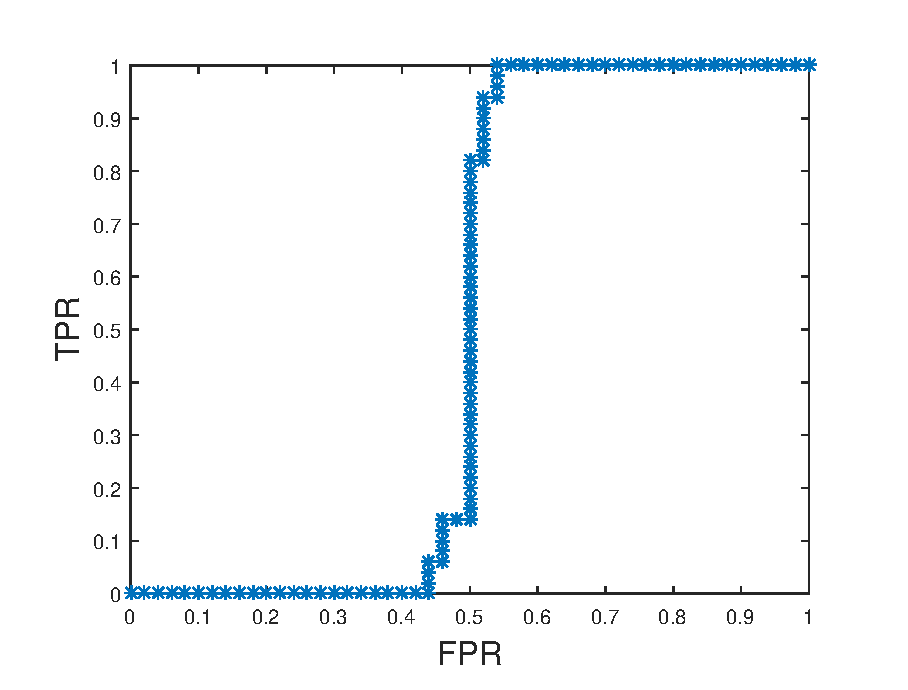
\includegraphics[width=0.6\textwidth]{figuras/prueba.eps}
	\caption{Pie de figura. Poner aquí cita del lugar de donde 
	se ha tomado la imagen en caso de que sea así. }
	\label{fig:prueba}
\end{figure}
\end{verbatim}

% Y ahora pongo la plantilla para que se incluya la figura efectivamente
\begin{figure}[t]
	\centering
	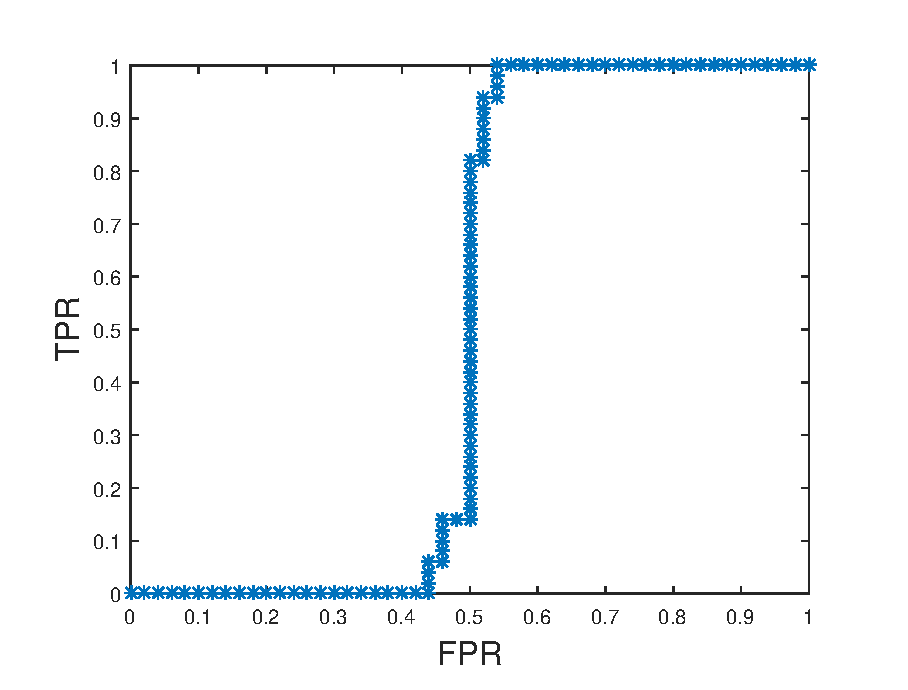
\includegraphics[width=0.6\textwidth]{figuras/prueba.eps}
	\caption{Pie de figura. Poner aquí cita del lugar de donde se ha tomado la imagen en caso de que sea así. }
	\label{fig:prueba}
\end{figure}

Si se pone el modificador [t] (top) latex ubicará la figura en la parte de arriba de la página. Ver otros modificadores como [h] (here) o [b] (bottom). Se pueden usar otras plantillas para, por ejemplo, poner dos figuras una al lado de otra. Consultar en Internet diferentes plantillas en caso de necesidad. 

Cuando en el texto nos refiramos a la figura en cuestión por el número, debemos usar la mayúscula y utilizar referencia a la figura. Esto hará que no nos tengamos que preocupar de la numeración de las figuras. Ej. Como se puede comprobar en la Figura~\ref{fig:prueba}.

Sustituir expresiones del tipo: “En la siguiente figura…” por “En la Figura 2.2…”


\subsection*{Inserción de tablas}

Este sería un ejemplo de una tabla. Se puede modificar el formato y contenido (ver en Internet algún enlace sobre cómo formatear tablas en latex). 

\begin{table}[t]
	\caption{Descripción de la tabla.}
	\label{table:prueba}
	\centering
	\begin{tabular}{l  c} 
		\hline \\[-1.5ex]
		\textbf{Tipo de ataque} & \textbf{Etiqueta} \\ [1ex] 
		\hline\hline \\[-1.5ex]
		DoS11 & dos \\ [0.5ex]
		Exf1MBp & exf1KB \\ [1ex]
		\hline
	\end{tabular}
\end{table}

La forma de referirse a las tablas es similar a las de las figuras (usar mayúsculas y referencia a la etiqueta(label) de la tabla). Ej. Como se puede ver en la Tabla~\ref{table:prueba}, ...


\subsection*{Citas de bibliografía}
Ejemplo de cita de bibliografía. Primero se va a google.scholar y se busca la referencia. Después se da al enlace citar, y se elige el formato bibtex. Se copia ese texto en el fichero bibliografia.bib. Un ejemplo de referenciar una cita es \cite{macia2008evaluation}.


\subsection*{Referencias a secciones}

Para referirnos a secciones, primero debemos tener una etiqueta de tipo \texttt{label} en dicha sección. Posteriormente, pondremos una referencia a dicho label, igual que hacemos para las figuras y las tablas. Ej. Como se ha mencionado en la Sección~\ref{sec:intro:motivacion} (Nótese que la palabra Sección va con mayúscula).

\subsection*{Glosario y acrónimos}

Cuando se utilice un acrónimo se debe definir en el fichero glosario/entradas\_glosario, tal y como está el ejemplo en dicho fichero. Al referirse en el texto se indicará así: \gls{svm} (ver que la primera vez lo pondrá completo). La segunda vez que se referencie a \gls{svm} ya no aparece completo. También se puede nombrar en plural así: \glspl{svm}. 
Otros ejemplos de acrónimo son: \gls{gcd}, \gls{lcm}, \gls{gmf}. 

A la hora de compilar con el glosario, se debe abrir una terminal CMD en el directorio de los fuentes latex del proyecto, y ejecutar el siguiente comando: \texttt{makeglossaries proyecto}. Esto generará los ficheros auxiliares que contienen el glosario. 

\subsection*{Listados de código}

Aquí se puede ver un ejemplo de listado de código: 

%\begin{lstlisting}[frame=none, numbers=none]


\begin{lstlisting}[language=Python,caption=Ejemplo de Python, label=listado:pythonPrueba]
import numpy as np

def incmatrix(genl1,genl2):
	m = len(genl1)
	n = len(genl2)
	M = None #to become the incidence matrix
	VT = np.zeros((n*m,1), int)  #dummy variable

	#compute the bitwise xor matrix
	M1 = bitxormatrix(genl1)
	M2 = np.triu(bitxormatrix(genl2),1) 
	
	for i in range(m-1):
		for j in range(i+1, m):
			[r,c] = np.where(M2 == M1[i,j])
			for k in range(len(r)):
				VT[(i)*n + r[k]] = 1;
				VT[(i)*n + c[k]] = 1;
				VT[(j)*n + r[k]] = 1;
				VT[(j)*n + c[k]] = 1;
	
	if M is None:
		M = np.copy(VT)
	else:
		M = np.concatenate((M, VT), 1)
	
	VT = np.zeros((n*m,1), int)
	
	return M

\end{lstlisting}

Nos podemos referir a él como Listado de código~\ref{listado:pythonPrueba}. 
Si queremos que aparezca como un flotante en la página debemos poner la palabra \texttt{float} así: 
\begin{verbatim}
\begin{lstlisting}[float,language=Python,caption=Ejemplo de Python, 
label=listado:pythonPrueba]
\end{verbatim}


\subsection*{Enlaces URL}
Podemos poner un enlace así \url{http://dtstc.ugr.es/~gmacia}
\end{verbatim}

\section*{Recomendaciones generales}
A la hora de escribir el TFG/TFM es importante seguir las siguientes recomendaciones: 

\begin{enumerate}
	\item La memoria debe realizarse con el \textbf{máximo cuidado}, y debe proporcionar de forma consistente -y por sí misma- una idea clara y concisa de lo que se ha realizado. 
	\item No debe tener errores tipográficos ni ortográficos. Este es un aspecto que penaliza muchísimo el trabajo en la evaluación del tribunal. 
	\item Siempre que se utilice alguna figura no elaborada por el autor del proyecto debe indicarse la fuente de la que se ha sacado mediante una cita en la bibliografía. 
	\item La lectura debe ser fluida. Por ello, dada la dificultad que tiene afrontar la escritura de un texto largo casi por primera vez, se recomienda elaborar un índice rellenando los títulos de los diferentes apartados de que constará este documento. En segundo lugar, para cada apartado, se indicarán a modo de resumen las diferentes ideas que se desarrollarán posteriormente (una línea de texto por idea). Después, se desarrollan las ideas (cada idea en un párrafo). Cuando se termina, se realiza una lectura completa y detallada del texto para comprobar que es coherente y no tiene fallos ortográficos, tipográficos ni gramaticales, antes de pasarlo al tutor. 
	\item Una extensión normal está entorno a las 100-120 páginas. Esto no quiere decir que tengamos que escribir por escribir, ni meter contenido adicional sin sentido. Hay que escribir el proyecto de forma coherente, pero sin ser telegráfico, esto es, realizando una descripción detallada del trabajo realizado. 
	\item Evitar afirmaciones del tipo “El sistema diseñado es bastante bueno”. Esa misma frase debería ser escrita tal que responda a las preguntas: ¿Qué parte del sistema? ¿En qué sentido? ¿Cuánto de bueno? ¿Comparado con qué?
	\item Evitar la primera persona (incluso del plural). No obstante para resaltar la autoría de algo o enfatizar una posición personal sí se puede usar.
	\item Numerar estructuradamente los capítulos, secciones y subsecciones. Evitar más de tres niveles de anidamiento. 
	\item Toda afirmación categórica o se demuestra (teórica o experimentalmente)  o se incluye una referencia en la que se haya previamente demostrado.
	\item Toda tecnología, teorema, institución, norma, documento que se mencione debe estar referenciado. No incluir referencias a la wiki.
	\item Los términos en ingles que no tenga sentido traducir se pondrán en cursiva al menos para indicar que es un término no castellano.
	 

\end{enumerate}

\section*{Recomendaciones específicas para determinados contenidos}

\subsection*{Inserción de figuras}
Esta es una plantilla de código para adjuntar una figura. 

% El verbatim es solo para poner en el PDF el código que corresponde a la inserción de la figura
\begin{verbatim}
\begin{figure}[t]
	\centering
		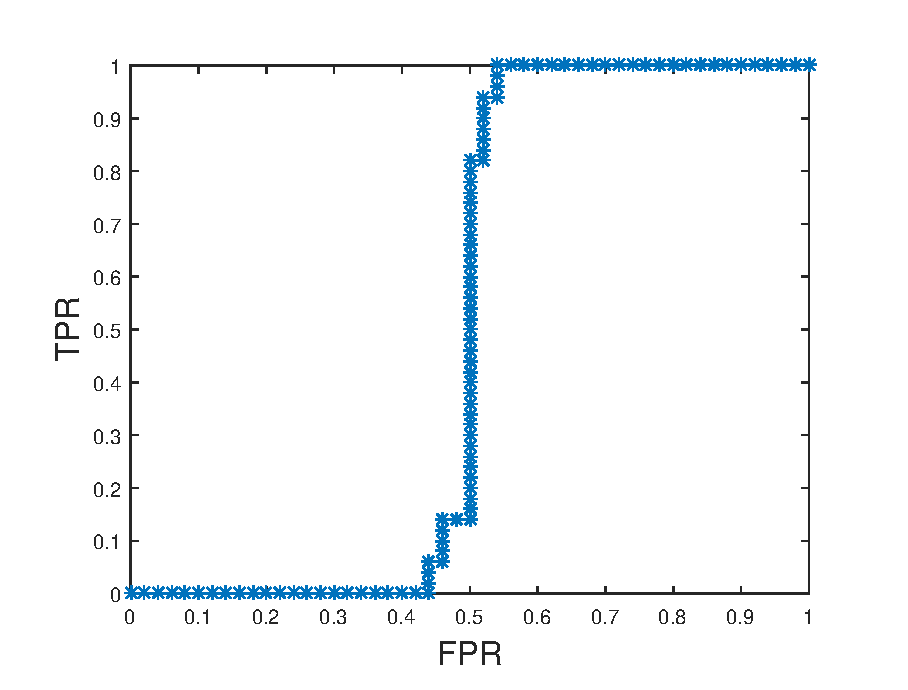
\includegraphics[width=0.6\textwidth]{figuras/prueba.eps}
	\caption{Pie de figura. Poner aquí cita del lugar de donde 
	se ha tomado la imagen en caso de que sea así. }
	\label{fig:prueba}
\end{figure}
\end{verbatim}

% Y ahora pongo la plantilla para que se incluya la figura efectivamente
\begin{figure}[t]
	\centering
	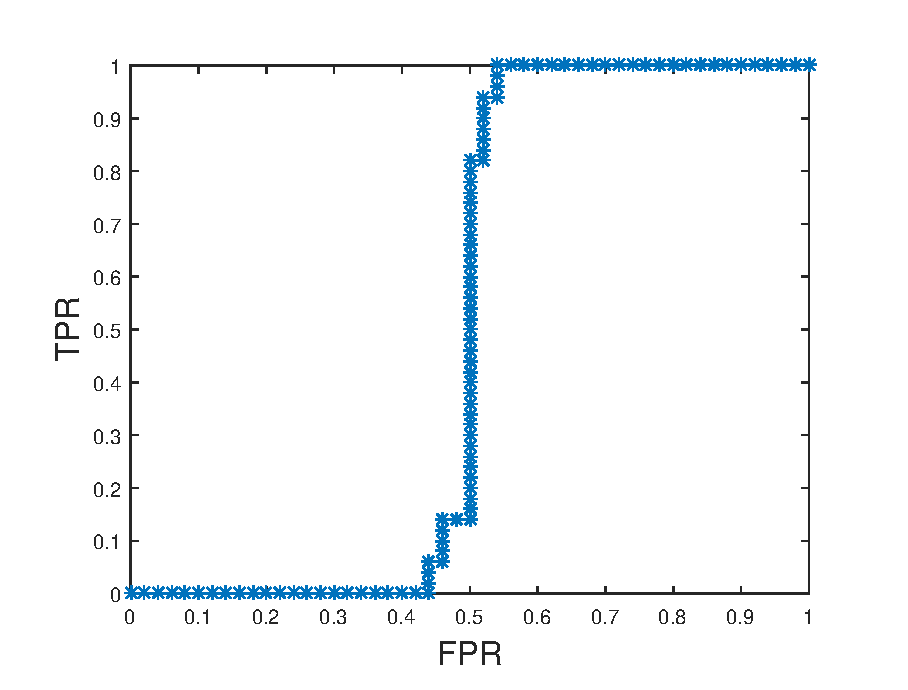
\includegraphics[width=0.6\textwidth]{figuras/prueba.eps}
	\caption{Pie de figura. Poner aquí cita del lugar de donde se ha tomado la imagen en caso de que sea así. }
	\label{fig:prueba}
\end{figure}

Si se pone el modificador [t] (top) latex ubicará la figura en la parte de arriba de la página. Ver otros modificadores como [h] (here) o [b] (bottom). Se pueden usar otras plantillas para, por ejemplo, poner dos figuras una al lado de otra. Consultar en Internet diferentes plantillas en caso de necesidad. 

Cuando en el texto nos refiramos a la figura en cuestión por el número, debemos usar la mayúscula y utilizar referencia a la figura. Esto hará que no nos tengamos que preocupar de la numeración de las figuras. Ej. Como se puede comprobar en la Figura~\ref{fig:prueba}.

Sustituir expresiones del tipo: “En la siguiente figura…” por “En la Figura 2.2…”


\subsection*{Inserción de tablas}

Este sería un ejemplo de una tabla. Se puede modificar el formato y contenido (ver en Internet algún enlace sobre cómo formatear tablas en latex). 

\begin{table}[t]
	\caption{Descripción de la tabla.}
	\label{table:prueba}
	\centering
	\begin{tabular}{l  c} 
		\hline \\[-1.5ex]
		\textbf{Tipo de ataque} & \textbf{Etiqueta} \\ [1ex] 
		\hline\hline \\[-1.5ex]
		DoS11 & dos \\ [0.5ex]
		Exf1MBp & exf1KB \\ [1ex]
		\hline
	\end{tabular}
\end{table}

La forma de referirse a las tablas es similar a las de las figuras (usar mayúsculas y referencia a la etiqueta(label) de la tabla). Ej. Como se puede ver en la Tabla~\ref{table:prueba}, ...


\subsection*{Citas de bibliografía}
Ejemplo de cita de bibliografía. Primero se va a google.scholar y se busca la referencia. Después se da al enlace citar, y se elige el formato bibtex. Se copia ese texto en el fichero bibliografia.bib. Un ejemplo de referenciar una cita es \cite{macia2008evaluation}.


\subsection*{Referencias a secciones}

Para referirnos a secciones, primero debemos tener una etiqueta de tipo \texttt{label} en dicha sección. Posteriormente, pondremos una referencia a dicho label, igual que hacemos para las figuras y las tablas. Ej. Como se ha mencionado en la Sección~\ref{sec:intro:motivacion} (Nótese que la palabra Sección va con mayúscula).

\subsection*{Glosario y acrónimos}

Cuando se utilice un acrónimo se debe definir en el fichero glosario/entradas\_glosario, tal y como está el ejemplo en dicho fichero. Al referirse en el texto se indicará así: \gls{svm} (ver que la primera vez lo pondrá completo). La segunda vez que se referencie a \gls{svm} ya no aparece completo. También se puede nombrar en plural así: \glspl{svm}. 
Otros ejemplos de acrónimo son: \gls{gcd}, \gls{lcm}, \gls{gmf}. 

A la hora de compilar con el glosario, se debe abrir una terminal CMD en el directorio de los fuentes latex del proyecto, y ejecutar el siguiente comando: \texttt{makeglossaries proyecto}. Esto generará los ficheros auxiliares que contienen el glosario. 

\subsection*{Listados de código}

Aquí se puede ver un ejemplo de listado de código: 

%\begin{lstlisting}[frame=none, numbers=none]


\begin{lstlisting}[language=Python,caption=Ejemplo de Python, label=listado:pythonPrueba]
import numpy as np

def incmatrix(genl1,genl2):
	m = len(genl1)
	n = len(genl2)
	M = None #to become the incidence matrix
	VT = np.zeros((n*m,1), int)  #dummy variable

	#compute the bitwise xor matrix
	M1 = bitxormatrix(genl1)
	M2 = np.triu(bitxormatrix(genl2),1) 
	
	for i in range(m-1):
		for j in range(i+1, m):
			[r,c] = np.where(M2 == M1[i,j])
			for k in range(len(r)):
				VT[(i)*n + r[k]] = 1;
				VT[(i)*n + c[k]] = 1;
				VT[(j)*n + r[k]] = 1;
				VT[(j)*n + c[k]] = 1;
	
	if M is None:
		M = np.copy(VT)
	else:
		M = np.concatenate((M, VT), 1)
	
	VT = np.zeros((n*m,1), int)
	
	return M

\end{lstlisting}

Nos podemos referir a él como Listado de código~\ref{listado:pythonPrueba}. 
Si queremos que aparezca como un flotante en la página debemos poner la palabra \texttt{float} así: 
\begin{verbatim}
\begin{lstlisting}[float,language=Python,caption=Ejemplo de Python, 
label=listado:pythonPrueba]
\end{verbatim}


\subsection*{Enlaces URL}
Podemos poner un enlace así \url{http://dtstc.ugr.es/~gmacia} --> %

\chapter*{Guía de estilo para escribir un TFG/TFM} \addcontentsline{toc}{chapter}{Guía de estilo}

Este capítulo no forma parte del TFG/TFM. Su único objetivo es aportar algunas recomendaciones y plantillas para tener claro cómo redactar el TFG/TFM. Una vez se haya comprendido, se puede comentar la siguiente línea en el fichero proyecto.tex añadiéndole al principio el carácter \%: 
\begin{verbatim}


\chapter*{Guía de estilo para escribir un TFG/TFM} \addcontentsline{toc}{chapter}{Guía de estilo}

Este capítulo no forma parte del TFG/TFM. Su único objetivo es aportar algunas recomendaciones y plantillas para tener claro cómo redactar el TFG/TFM. Una vez se haya comprendido, se puede comentar la siguiente línea en el fichero proyecto.tex añadiéndole al principio el carácter \%: 
\begin{verbatim}


\chapter*{Guía de estilo para escribir un TFG/TFM} \addcontentsline{toc}{chapter}{Guía de estilo}

Este capítulo no forma parte del TFG/TFM. Su único objetivo es aportar algunas recomendaciones y plantillas para tener claro cómo redactar el TFG/TFM. Una vez se haya comprendido, se puede comentar la siguiente línea en el fichero proyecto.tex añadiéndole al principio el carácter \%: 
\begin{verbatim}
\input{guiaDeEstilo} --> %\input{guiaDeEstilo}
\end{verbatim}

\section*{Recomendaciones generales}
A la hora de escribir el TFG/TFM es importante seguir las siguientes recomendaciones: 

\begin{enumerate}
	\item La memoria debe realizarse con el \textbf{máximo cuidado}, y debe proporcionar de forma consistente -y por sí misma- una idea clara y concisa de lo que se ha realizado. 
	\item No debe tener errores tipográficos ni ortográficos. Este es un aspecto que penaliza muchísimo el trabajo en la evaluación del tribunal. 
	\item Siempre que se utilice alguna figura no elaborada por el autor del proyecto debe indicarse la fuente de la que se ha sacado mediante una cita en la bibliografía. 
	\item La lectura debe ser fluida. Por ello, dada la dificultad que tiene afrontar la escritura de un texto largo casi por primera vez, se recomienda elaborar un índice rellenando los títulos de los diferentes apartados de que constará este documento. En segundo lugar, para cada apartado, se indicarán a modo de resumen las diferentes ideas que se desarrollarán posteriormente (una línea de texto por idea). Después, se desarrollan las ideas (cada idea en un párrafo). Cuando se termina, se realiza una lectura completa y detallada del texto para comprobar que es coherente y no tiene fallos ortográficos, tipográficos ni gramaticales, antes de pasarlo al tutor. 
	\item Una extensión normal está entorno a las 100-120 páginas. Esto no quiere decir que tengamos que escribir por escribir, ni meter contenido adicional sin sentido. Hay que escribir el proyecto de forma coherente, pero sin ser telegráfico, esto es, realizando una descripción detallada del trabajo realizado. 
	\item Evitar afirmaciones del tipo “El sistema diseñado es bastante bueno”. Esa misma frase debería ser escrita tal que responda a las preguntas: ¿Qué parte del sistema? ¿En qué sentido? ¿Cuánto de bueno? ¿Comparado con qué?
	\item Evitar la primera persona (incluso del plural). No obstante para resaltar la autoría de algo o enfatizar una posición personal sí se puede usar.
	\item Numerar estructuradamente los capítulos, secciones y subsecciones. Evitar más de tres niveles de anidamiento. 
	\item Toda afirmación categórica o se demuestra (teórica o experimentalmente)  o se incluye una referencia en la que se haya previamente demostrado.
	\item Toda tecnología, teorema, institución, norma, documento que se mencione debe estar referenciado. No incluir referencias a la wiki.
	\item Los términos en ingles que no tenga sentido traducir se pondrán en cursiva al menos para indicar que es un término no castellano.
	 

\end{enumerate}

\section*{Recomendaciones específicas para determinados contenidos}

\subsection*{Inserción de figuras}
Esta es una plantilla de código para adjuntar una figura. 

% El verbatim es solo para poner en el PDF el código que corresponde a la inserción de la figura
\begin{verbatim}
\begin{figure}[t]
	\centering
		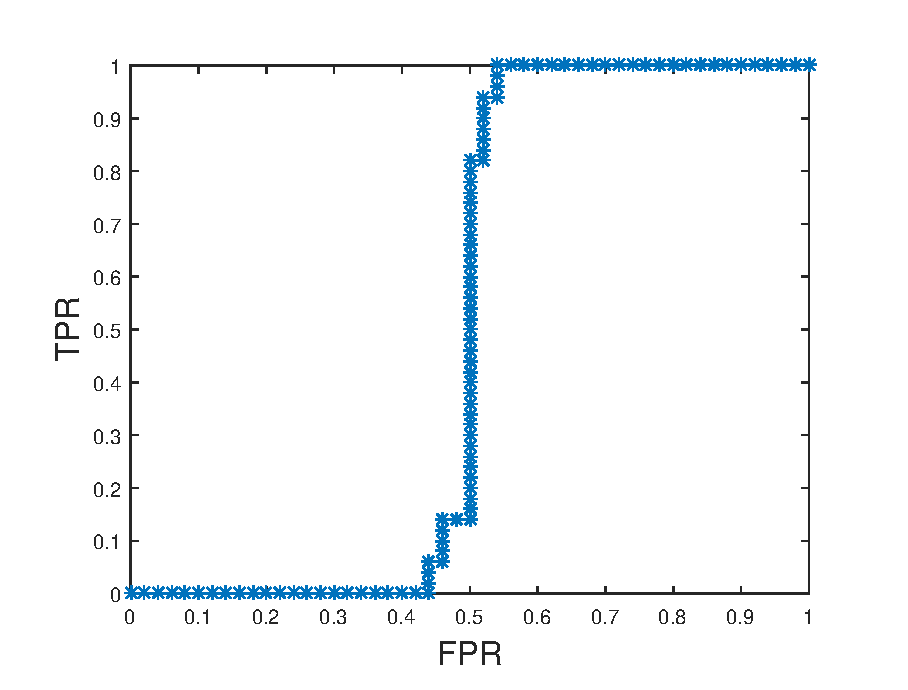
\includegraphics[width=0.6\textwidth]{figuras/prueba.eps}
	\caption{Pie de figura. Poner aquí cita del lugar de donde 
	se ha tomado la imagen en caso de que sea así. }
	\label{fig:prueba}
\end{figure}
\end{verbatim}

% Y ahora pongo la plantilla para que se incluya la figura efectivamente
\begin{figure}[t]
	\centering
	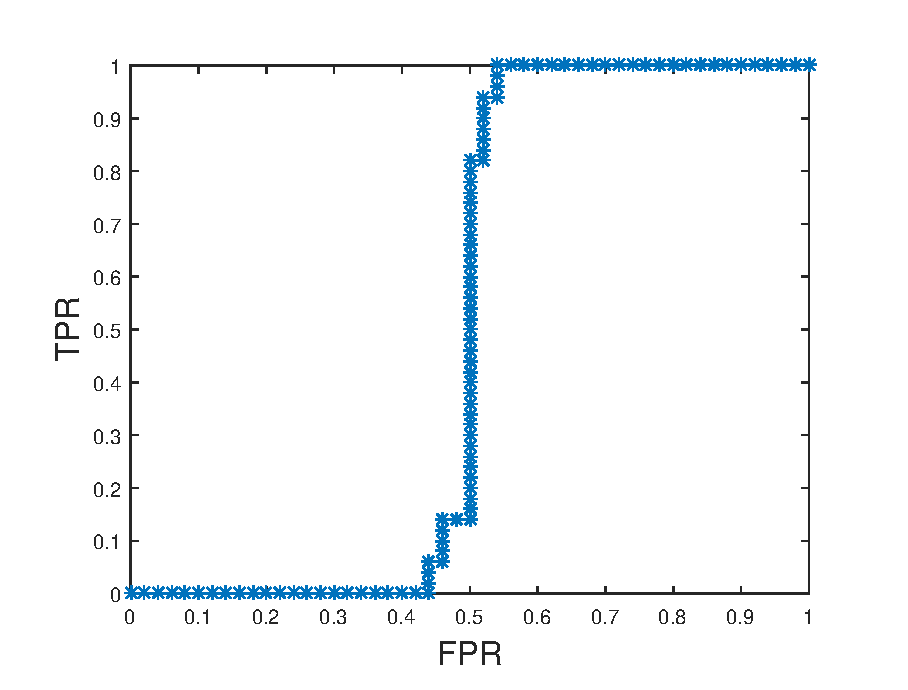
\includegraphics[width=0.6\textwidth]{figuras/prueba.eps}
	\caption{Pie de figura. Poner aquí cita del lugar de donde se ha tomado la imagen en caso de que sea así. }
	\label{fig:prueba}
\end{figure}

Si se pone el modificador [t] (top) latex ubicará la figura en la parte de arriba de la página. Ver otros modificadores como [h] (here) o [b] (bottom). Se pueden usar otras plantillas para, por ejemplo, poner dos figuras una al lado de otra. Consultar en Internet diferentes plantillas en caso de necesidad. 

Cuando en el texto nos refiramos a la figura en cuestión por el número, debemos usar la mayúscula y utilizar referencia a la figura. Esto hará que no nos tengamos que preocupar de la numeración de las figuras. Ej. Como se puede comprobar en la Figura~\ref{fig:prueba}.

Sustituir expresiones del tipo: “En la siguiente figura…” por “En la Figura 2.2…”


\subsection*{Inserción de tablas}

Este sería un ejemplo de una tabla. Se puede modificar el formato y contenido (ver en Internet algún enlace sobre cómo formatear tablas en latex). 

\begin{table}[t]
	\caption{Descripción de la tabla.}
	\label{table:prueba}
	\centering
	\begin{tabular}{l  c} 
		\hline \\[-1.5ex]
		\textbf{Tipo de ataque} & \textbf{Etiqueta} \\ [1ex] 
		\hline\hline \\[-1.5ex]
		DoS11 & dos \\ [0.5ex]
		Exf1MBp & exf1KB \\ [1ex]
		\hline
	\end{tabular}
\end{table}

La forma de referirse a las tablas es similar a las de las figuras (usar mayúsculas y referencia a la etiqueta(label) de la tabla). Ej. Como se puede ver en la Tabla~\ref{table:prueba}, ...


\subsection*{Citas de bibliografía}
Ejemplo de cita de bibliografía. Primero se va a google.scholar y se busca la referencia. Después se da al enlace citar, y se elige el formato bibtex. Se copia ese texto en el fichero bibliografia.bib. Un ejemplo de referenciar una cita es \cite{macia2008evaluation}.


\subsection*{Referencias a secciones}

Para referirnos a secciones, primero debemos tener una etiqueta de tipo \texttt{label} en dicha sección. Posteriormente, pondremos una referencia a dicho label, igual que hacemos para las figuras y las tablas. Ej. Como se ha mencionado en la Sección~\ref{sec:intro:motivacion} (Nótese que la palabra Sección va con mayúscula).

\subsection*{Glosario y acrónimos}

Cuando se utilice un acrónimo se debe definir en el fichero glosario/entradas\_glosario, tal y como está el ejemplo en dicho fichero. Al referirse en el texto se indicará así: \gls{svm} (ver que la primera vez lo pondrá completo). La segunda vez que se referencie a \gls{svm} ya no aparece completo. También se puede nombrar en plural así: \glspl{svm}. 
Otros ejemplos de acrónimo son: \gls{gcd}, \gls{lcm}, \gls{gmf}. 

A la hora de compilar con el glosario, se debe abrir una terminal CMD en el directorio de los fuentes latex del proyecto, y ejecutar el siguiente comando: \texttt{makeglossaries proyecto}. Esto generará los ficheros auxiliares que contienen el glosario. 

\subsection*{Listados de código}

Aquí se puede ver un ejemplo de listado de código: 

%\begin{lstlisting}[frame=none, numbers=none]


\begin{lstlisting}[language=Python,caption=Ejemplo de Python, label=listado:pythonPrueba]
import numpy as np

def incmatrix(genl1,genl2):
	m = len(genl1)
	n = len(genl2)
	M = None #to become the incidence matrix
	VT = np.zeros((n*m,1), int)  #dummy variable

	#compute the bitwise xor matrix
	M1 = bitxormatrix(genl1)
	M2 = np.triu(bitxormatrix(genl2),1) 
	
	for i in range(m-1):
		for j in range(i+1, m):
			[r,c] = np.where(M2 == M1[i,j])
			for k in range(len(r)):
				VT[(i)*n + r[k]] = 1;
				VT[(i)*n + c[k]] = 1;
				VT[(j)*n + r[k]] = 1;
				VT[(j)*n + c[k]] = 1;
	
	if M is None:
		M = np.copy(VT)
	else:
		M = np.concatenate((M, VT), 1)
	
	VT = np.zeros((n*m,1), int)
	
	return M

\end{lstlisting}

Nos podemos referir a él como Listado de código~\ref{listado:pythonPrueba}. 
Si queremos que aparezca como un flotante en la página debemos poner la palabra \texttt{float} así: 
\begin{verbatim}
\begin{lstlisting}[float,language=Python,caption=Ejemplo de Python, 
label=listado:pythonPrueba]
\end{verbatim}


\subsection*{Enlaces URL}
Podemos poner un enlace así \url{http://dtstc.ugr.es/~gmacia} --> %

\chapter*{Guía de estilo para escribir un TFG/TFM} \addcontentsline{toc}{chapter}{Guía de estilo}

Este capítulo no forma parte del TFG/TFM. Su único objetivo es aportar algunas recomendaciones y plantillas para tener claro cómo redactar el TFG/TFM. Una vez se haya comprendido, se puede comentar la siguiente línea en el fichero proyecto.tex añadiéndole al principio el carácter \%: 
\begin{verbatim}
\input{guiaDeEstilo} --> %\input{guiaDeEstilo}
\end{verbatim}

\section*{Recomendaciones generales}
A la hora de escribir el TFG/TFM es importante seguir las siguientes recomendaciones: 

\begin{enumerate}
	\item La memoria debe realizarse con el \textbf{máximo cuidado}, y debe proporcionar de forma consistente -y por sí misma- una idea clara y concisa de lo que se ha realizado. 
	\item No debe tener errores tipográficos ni ortográficos. Este es un aspecto que penaliza muchísimo el trabajo en la evaluación del tribunal. 
	\item Siempre que se utilice alguna figura no elaborada por el autor del proyecto debe indicarse la fuente de la que se ha sacado mediante una cita en la bibliografía. 
	\item La lectura debe ser fluida. Por ello, dada la dificultad que tiene afrontar la escritura de un texto largo casi por primera vez, se recomienda elaborar un índice rellenando los títulos de los diferentes apartados de que constará este documento. En segundo lugar, para cada apartado, se indicarán a modo de resumen las diferentes ideas que se desarrollarán posteriormente (una línea de texto por idea). Después, se desarrollan las ideas (cada idea en un párrafo). Cuando se termina, se realiza una lectura completa y detallada del texto para comprobar que es coherente y no tiene fallos ortográficos, tipográficos ni gramaticales, antes de pasarlo al tutor. 
	\item Una extensión normal está entorno a las 100-120 páginas. Esto no quiere decir que tengamos que escribir por escribir, ni meter contenido adicional sin sentido. Hay que escribir el proyecto de forma coherente, pero sin ser telegráfico, esto es, realizando una descripción detallada del trabajo realizado. 
	\item Evitar afirmaciones del tipo “El sistema diseñado es bastante bueno”. Esa misma frase debería ser escrita tal que responda a las preguntas: ¿Qué parte del sistema? ¿En qué sentido? ¿Cuánto de bueno? ¿Comparado con qué?
	\item Evitar la primera persona (incluso del plural). No obstante para resaltar la autoría de algo o enfatizar una posición personal sí se puede usar.
	\item Numerar estructuradamente los capítulos, secciones y subsecciones. Evitar más de tres niveles de anidamiento. 
	\item Toda afirmación categórica o se demuestra (teórica o experimentalmente)  o se incluye una referencia en la que se haya previamente demostrado.
	\item Toda tecnología, teorema, institución, norma, documento que se mencione debe estar referenciado. No incluir referencias a la wiki.
	\item Los términos en ingles que no tenga sentido traducir se pondrán en cursiva al menos para indicar que es un término no castellano.
	 

\end{enumerate}

\section*{Recomendaciones específicas para determinados contenidos}

\subsection*{Inserción de figuras}
Esta es una plantilla de código para adjuntar una figura. 

% El verbatim es solo para poner en el PDF el código que corresponde a la inserción de la figura
\begin{verbatim}
\begin{figure}[t]
	\centering
		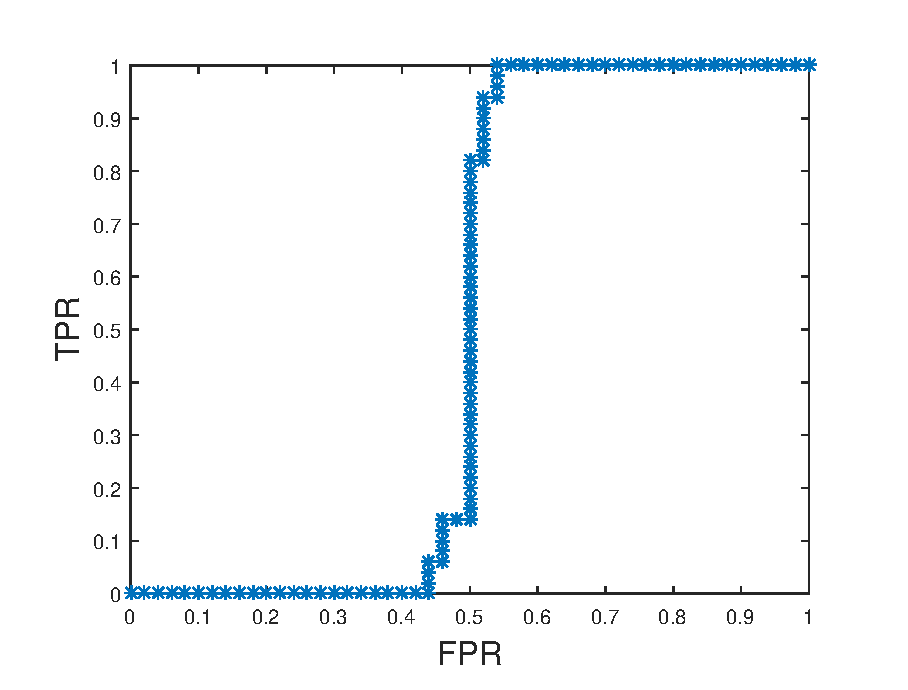
\includegraphics[width=0.6\textwidth]{figuras/prueba.eps}
	\caption{Pie de figura. Poner aquí cita del lugar de donde 
	se ha tomado la imagen en caso de que sea así. }
	\label{fig:prueba}
\end{figure}
\end{verbatim}

% Y ahora pongo la plantilla para que se incluya la figura efectivamente
\begin{figure}[t]
	\centering
	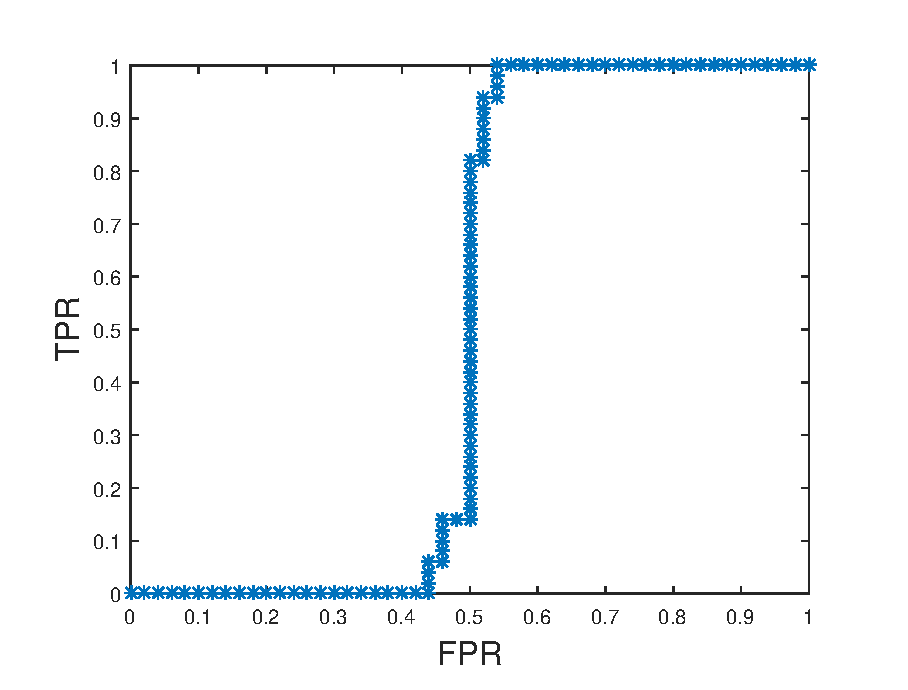
\includegraphics[width=0.6\textwidth]{figuras/prueba.eps}
	\caption{Pie de figura. Poner aquí cita del lugar de donde se ha tomado la imagen en caso de que sea así. }
	\label{fig:prueba}
\end{figure}

Si se pone el modificador [t] (top) latex ubicará la figura en la parte de arriba de la página. Ver otros modificadores como [h] (here) o [b] (bottom). Se pueden usar otras plantillas para, por ejemplo, poner dos figuras una al lado de otra. Consultar en Internet diferentes plantillas en caso de necesidad. 

Cuando en el texto nos refiramos a la figura en cuestión por el número, debemos usar la mayúscula y utilizar referencia a la figura. Esto hará que no nos tengamos que preocupar de la numeración de las figuras. Ej. Como se puede comprobar en la Figura~\ref{fig:prueba}.

Sustituir expresiones del tipo: “En la siguiente figura…” por “En la Figura 2.2…”


\subsection*{Inserción de tablas}

Este sería un ejemplo de una tabla. Se puede modificar el formato y contenido (ver en Internet algún enlace sobre cómo formatear tablas en latex). 

\begin{table}[t]
	\caption{Descripción de la tabla.}
	\label{table:prueba}
	\centering
	\begin{tabular}{l  c} 
		\hline \\[-1.5ex]
		\textbf{Tipo de ataque} & \textbf{Etiqueta} \\ [1ex] 
		\hline\hline \\[-1.5ex]
		DoS11 & dos \\ [0.5ex]
		Exf1MBp & exf1KB \\ [1ex]
		\hline
	\end{tabular}
\end{table}

La forma de referirse a las tablas es similar a las de las figuras (usar mayúsculas y referencia a la etiqueta(label) de la tabla). Ej. Como se puede ver en la Tabla~\ref{table:prueba}, ...


\subsection*{Citas de bibliografía}
Ejemplo de cita de bibliografía. Primero se va a google.scholar y se busca la referencia. Después se da al enlace citar, y se elige el formato bibtex. Se copia ese texto en el fichero bibliografia.bib. Un ejemplo de referenciar una cita es \cite{macia2008evaluation}.


\subsection*{Referencias a secciones}

Para referirnos a secciones, primero debemos tener una etiqueta de tipo \texttt{label} en dicha sección. Posteriormente, pondremos una referencia a dicho label, igual que hacemos para las figuras y las tablas. Ej. Como se ha mencionado en la Sección~\ref{sec:intro:motivacion} (Nótese que la palabra Sección va con mayúscula).

\subsection*{Glosario y acrónimos}

Cuando se utilice un acrónimo se debe definir en el fichero glosario/entradas\_glosario, tal y como está el ejemplo en dicho fichero. Al referirse en el texto se indicará así: \gls{svm} (ver que la primera vez lo pondrá completo). La segunda vez que se referencie a \gls{svm} ya no aparece completo. También se puede nombrar en plural así: \glspl{svm}. 
Otros ejemplos de acrónimo son: \gls{gcd}, \gls{lcm}, \gls{gmf}. 

A la hora de compilar con el glosario, se debe abrir una terminal CMD en el directorio de los fuentes latex del proyecto, y ejecutar el siguiente comando: \texttt{makeglossaries proyecto}. Esto generará los ficheros auxiliares que contienen el glosario. 

\subsection*{Listados de código}

Aquí se puede ver un ejemplo de listado de código: 

%\begin{lstlisting}[frame=none, numbers=none]


\begin{lstlisting}[language=Python,caption=Ejemplo de Python, label=listado:pythonPrueba]
import numpy as np

def incmatrix(genl1,genl2):
	m = len(genl1)
	n = len(genl2)
	M = None #to become the incidence matrix
	VT = np.zeros((n*m,1), int)  #dummy variable

	#compute the bitwise xor matrix
	M1 = bitxormatrix(genl1)
	M2 = np.triu(bitxormatrix(genl2),1) 
	
	for i in range(m-1):
		for j in range(i+1, m):
			[r,c] = np.where(M2 == M1[i,j])
			for k in range(len(r)):
				VT[(i)*n + r[k]] = 1;
				VT[(i)*n + c[k]] = 1;
				VT[(j)*n + r[k]] = 1;
				VT[(j)*n + c[k]] = 1;
	
	if M is None:
		M = np.copy(VT)
	else:
		M = np.concatenate((M, VT), 1)
	
	VT = np.zeros((n*m,1), int)
	
	return M

\end{lstlisting}

Nos podemos referir a él como Listado de código~\ref{listado:pythonPrueba}. 
Si queremos que aparezca como un flotante en la página debemos poner la palabra \texttt{float} así: 
\begin{verbatim}
\begin{lstlisting}[float,language=Python,caption=Ejemplo de Python, 
label=listado:pythonPrueba]
\end{verbatim}


\subsection*{Enlaces URL}
Podemos poner un enlace así \url{http://dtstc.ugr.es/~gmacia}
\end{verbatim}

\section*{Recomendaciones generales}
A la hora de escribir el TFG/TFM es importante seguir las siguientes recomendaciones: 

\begin{enumerate}
	\item La memoria debe realizarse con el \textbf{máximo cuidado}, y debe proporcionar de forma consistente -y por sí misma- una idea clara y concisa de lo que se ha realizado. 
	\item No debe tener errores tipográficos ni ortográficos. Este es un aspecto que penaliza muchísimo el trabajo en la evaluación del tribunal. 
	\item Siempre que se utilice alguna figura no elaborada por el autor del proyecto debe indicarse la fuente de la que se ha sacado mediante una cita en la bibliografía. 
	\item La lectura debe ser fluida. Por ello, dada la dificultad que tiene afrontar la escritura de un texto largo casi por primera vez, se recomienda elaborar un índice rellenando los títulos de los diferentes apartados de que constará este documento. En segundo lugar, para cada apartado, se indicarán a modo de resumen las diferentes ideas que se desarrollarán posteriormente (una línea de texto por idea). Después, se desarrollan las ideas (cada idea en un párrafo). Cuando se termina, se realiza una lectura completa y detallada del texto para comprobar que es coherente y no tiene fallos ortográficos, tipográficos ni gramaticales, antes de pasarlo al tutor. 
	\item Una extensión normal está entorno a las 100-120 páginas. Esto no quiere decir que tengamos que escribir por escribir, ni meter contenido adicional sin sentido. Hay que escribir el proyecto de forma coherente, pero sin ser telegráfico, esto es, realizando una descripción detallada del trabajo realizado. 
	\item Evitar afirmaciones del tipo “El sistema diseñado es bastante bueno”. Esa misma frase debería ser escrita tal que responda a las preguntas: ¿Qué parte del sistema? ¿En qué sentido? ¿Cuánto de bueno? ¿Comparado con qué?
	\item Evitar la primera persona (incluso del plural). No obstante para resaltar la autoría de algo o enfatizar una posición personal sí se puede usar.
	\item Numerar estructuradamente los capítulos, secciones y subsecciones. Evitar más de tres niveles de anidamiento. 
	\item Toda afirmación categórica o se demuestra (teórica o experimentalmente)  o se incluye una referencia en la que se haya previamente demostrado.
	\item Toda tecnología, teorema, institución, norma, documento que se mencione debe estar referenciado. No incluir referencias a la wiki.
	\item Los términos en ingles que no tenga sentido traducir se pondrán en cursiva al menos para indicar que es un término no castellano.
	 

\end{enumerate}

\section*{Recomendaciones específicas para determinados contenidos}

\subsection*{Inserción de figuras}
Esta es una plantilla de código para adjuntar una figura. 

% El verbatim es solo para poner en el PDF el código que corresponde a la inserción de la figura
\begin{verbatim}
\begin{figure}[t]
	\centering
		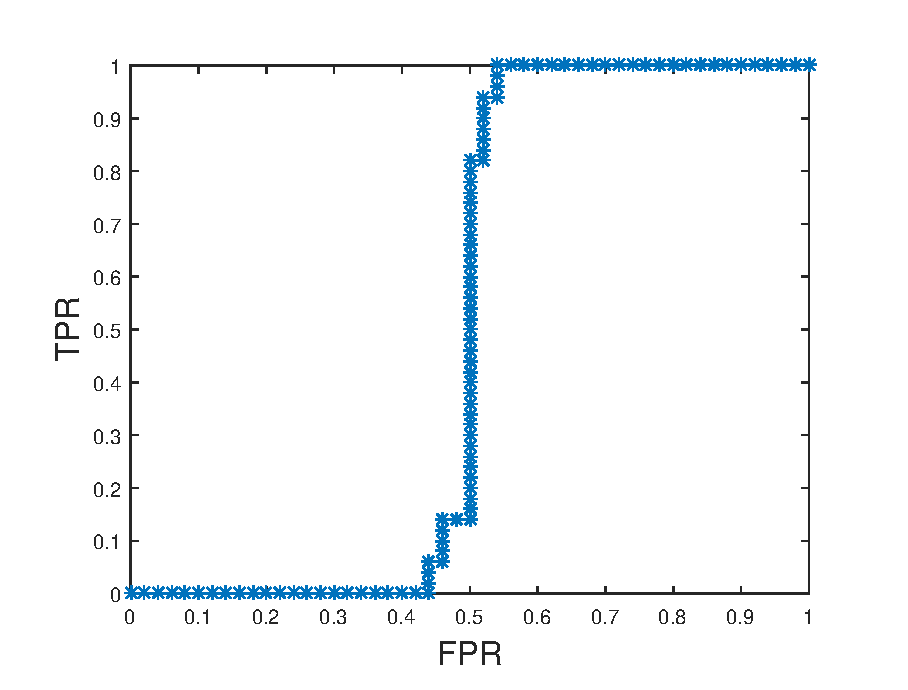
\includegraphics[width=0.6\textwidth]{figuras/prueba.eps}
	\caption{Pie de figura. Poner aquí cita del lugar de donde 
	se ha tomado la imagen en caso de que sea así. }
	\label{fig:prueba}
\end{figure}
\end{verbatim}

% Y ahora pongo la plantilla para que se incluya la figura efectivamente
\begin{figure}[t]
	\centering
	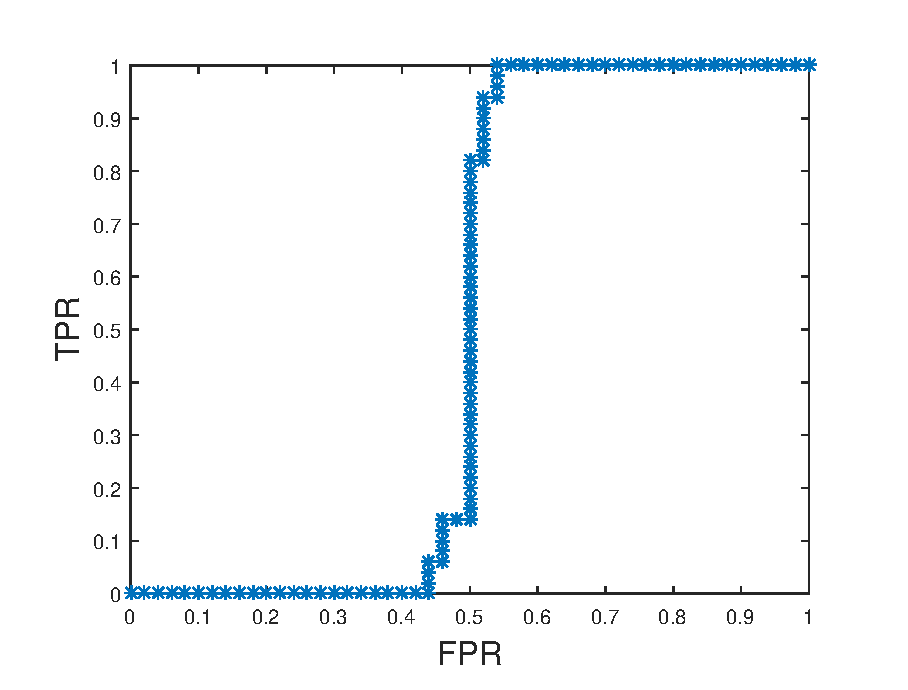
\includegraphics[width=0.6\textwidth]{figuras/prueba.eps}
	\caption{Pie de figura. Poner aquí cita del lugar de donde se ha tomado la imagen en caso de que sea así. }
	\label{fig:prueba}
\end{figure}

Si se pone el modificador [t] (top) latex ubicará la figura en la parte de arriba de la página. Ver otros modificadores como [h] (here) o [b] (bottom). Se pueden usar otras plantillas para, por ejemplo, poner dos figuras una al lado de otra. Consultar en Internet diferentes plantillas en caso de necesidad. 

Cuando en el texto nos refiramos a la figura en cuestión por el número, debemos usar la mayúscula y utilizar referencia a la figura. Esto hará que no nos tengamos que preocupar de la numeración de las figuras. Ej. Como se puede comprobar en la Figura~\ref{fig:prueba}.

Sustituir expresiones del tipo: “En la siguiente figura…” por “En la Figura 2.2…”


\subsection*{Inserción de tablas}

Este sería un ejemplo de una tabla. Se puede modificar el formato y contenido (ver en Internet algún enlace sobre cómo formatear tablas en latex). 

\begin{table}[t]
	\caption{Descripción de la tabla.}
	\label{table:prueba}
	\centering
	\begin{tabular}{l  c} 
		\hline \\[-1.5ex]
		\textbf{Tipo de ataque} & \textbf{Etiqueta} \\ [1ex] 
		\hline\hline \\[-1.5ex]
		DoS11 & dos \\ [0.5ex]
		Exf1MBp & exf1KB \\ [1ex]
		\hline
	\end{tabular}
\end{table}

La forma de referirse a las tablas es similar a las de las figuras (usar mayúsculas y referencia a la etiqueta(label) de la tabla). Ej. Como se puede ver en la Tabla~\ref{table:prueba}, ...


\subsection*{Citas de bibliografía}
Ejemplo de cita de bibliografía. Primero se va a google.scholar y se busca la referencia. Después se da al enlace citar, y se elige el formato bibtex. Se copia ese texto en el fichero bibliografia.bib. Un ejemplo de referenciar una cita es \cite{macia2008evaluation}.


\subsection*{Referencias a secciones}

Para referirnos a secciones, primero debemos tener una etiqueta de tipo \texttt{label} en dicha sección. Posteriormente, pondremos una referencia a dicho label, igual que hacemos para las figuras y las tablas. Ej. Como se ha mencionado en la Sección~\ref{sec:intro:motivacion} (Nótese que la palabra Sección va con mayúscula).

\subsection*{Glosario y acrónimos}

Cuando se utilice un acrónimo se debe definir en el fichero glosario/entradas\_glosario, tal y como está el ejemplo en dicho fichero. Al referirse en el texto se indicará así: \gls{svm} (ver que la primera vez lo pondrá completo). La segunda vez que se referencie a \gls{svm} ya no aparece completo. También se puede nombrar en plural así: \glspl{svm}. 
Otros ejemplos de acrónimo son: \gls{gcd}, \gls{lcm}, \gls{gmf}. 

A la hora de compilar con el glosario, se debe abrir una terminal CMD en el directorio de los fuentes latex del proyecto, y ejecutar el siguiente comando: \texttt{makeglossaries proyecto}. Esto generará los ficheros auxiliares que contienen el glosario. 

\subsection*{Listados de código}

Aquí se puede ver un ejemplo de listado de código: 

%\begin{lstlisting}[frame=none, numbers=none]


\begin{lstlisting}[language=Python,caption=Ejemplo de Python, label=listado:pythonPrueba]
import numpy as np

def incmatrix(genl1,genl2):
	m = len(genl1)
	n = len(genl2)
	M = None #to become the incidence matrix
	VT = np.zeros((n*m,1), int)  #dummy variable

	#compute the bitwise xor matrix
	M1 = bitxormatrix(genl1)
	M2 = np.triu(bitxormatrix(genl2),1) 
	
	for i in range(m-1):
		for j in range(i+1, m):
			[r,c] = np.where(M2 == M1[i,j])
			for k in range(len(r)):
				VT[(i)*n + r[k]] = 1;
				VT[(i)*n + c[k]] = 1;
				VT[(j)*n + r[k]] = 1;
				VT[(j)*n + c[k]] = 1;
	
	if M is None:
		M = np.copy(VT)
	else:
		M = np.concatenate((M, VT), 1)
	
	VT = np.zeros((n*m,1), int)
	
	return M

\end{lstlisting}

Nos podemos referir a él como Listado de código~\ref{listado:pythonPrueba}. 
Si queremos que aparezca como un flotante en la página debemos poner la palabra \texttt{float} así: 
\begin{verbatim}
\begin{lstlisting}[float,language=Python,caption=Ejemplo de Python, 
label=listado:pythonPrueba]
\end{verbatim}


\subsection*{Enlaces URL}
Podemos poner un enlace así \url{http://dtstc.ugr.es/~gmacia} --> %

\chapter*{Guía de estilo para escribir un TFG/TFM} \addcontentsline{toc}{chapter}{Guía de estilo}

Este capítulo no forma parte del TFG/TFM. Su único objetivo es aportar algunas recomendaciones y plantillas para tener claro cómo redactar el TFG/TFM. Una vez se haya comprendido, se puede comentar la siguiente línea en el fichero proyecto.tex añadiéndole al principio el carácter \%: 
\begin{verbatim}


\chapter*{Guía de estilo para escribir un TFG/TFM} \addcontentsline{toc}{chapter}{Guía de estilo}

Este capítulo no forma parte del TFG/TFM. Su único objetivo es aportar algunas recomendaciones y plantillas para tener claro cómo redactar el TFG/TFM. Una vez se haya comprendido, se puede comentar la siguiente línea en el fichero proyecto.tex añadiéndole al principio el carácter \%: 
\begin{verbatim}
\input{guiaDeEstilo} --> %\input{guiaDeEstilo}
\end{verbatim}

\section*{Recomendaciones generales}
A la hora de escribir el TFG/TFM es importante seguir las siguientes recomendaciones: 

\begin{enumerate}
	\item La memoria debe realizarse con el \textbf{máximo cuidado}, y debe proporcionar de forma consistente -y por sí misma- una idea clara y concisa de lo que se ha realizado. 
	\item No debe tener errores tipográficos ni ortográficos. Este es un aspecto que penaliza muchísimo el trabajo en la evaluación del tribunal. 
	\item Siempre que se utilice alguna figura no elaborada por el autor del proyecto debe indicarse la fuente de la que se ha sacado mediante una cita en la bibliografía. 
	\item La lectura debe ser fluida. Por ello, dada la dificultad que tiene afrontar la escritura de un texto largo casi por primera vez, se recomienda elaborar un índice rellenando los títulos de los diferentes apartados de que constará este documento. En segundo lugar, para cada apartado, se indicarán a modo de resumen las diferentes ideas que se desarrollarán posteriormente (una línea de texto por idea). Después, se desarrollan las ideas (cada idea en un párrafo). Cuando se termina, se realiza una lectura completa y detallada del texto para comprobar que es coherente y no tiene fallos ortográficos, tipográficos ni gramaticales, antes de pasarlo al tutor. 
	\item Una extensión normal está entorno a las 100-120 páginas. Esto no quiere decir que tengamos que escribir por escribir, ni meter contenido adicional sin sentido. Hay que escribir el proyecto de forma coherente, pero sin ser telegráfico, esto es, realizando una descripción detallada del trabajo realizado. 
	\item Evitar afirmaciones del tipo “El sistema diseñado es bastante bueno”. Esa misma frase debería ser escrita tal que responda a las preguntas: ¿Qué parte del sistema? ¿En qué sentido? ¿Cuánto de bueno? ¿Comparado con qué?
	\item Evitar la primera persona (incluso del plural). No obstante para resaltar la autoría de algo o enfatizar una posición personal sí se puede usar.
	\item Numerar estructuradamente los capítulos, secciones y subsecciones. Evitar más de tres niveles de anidamiento. 
	\item Toda afirmación categórica o se demuestra (teórica o experimentalmente)  o se incluye una referencia en la que se haya previamente demostrado.
	\item Toda tecnología, teorema, institución, norma, documento que se mencione debe estar referenciado. No incluir referencias a la wiki.
	\item Los términos en ingles que no tenga sentido traducir se pondrán en cursiva al menos para indicar que es un término no castellano.
	 

\end{enumerate}

\section*{Recomendaciones específicas para determinados contenidos}

\subsection*{Inserción de figuras}
Esta es una plantilla de código para adjuntar una figura. 

% El verbatim es solo para poner en el PDF el código que corresponde a la inserción de la figura
\begin{verbatim}
\begin{figure}[t]
	\centering
		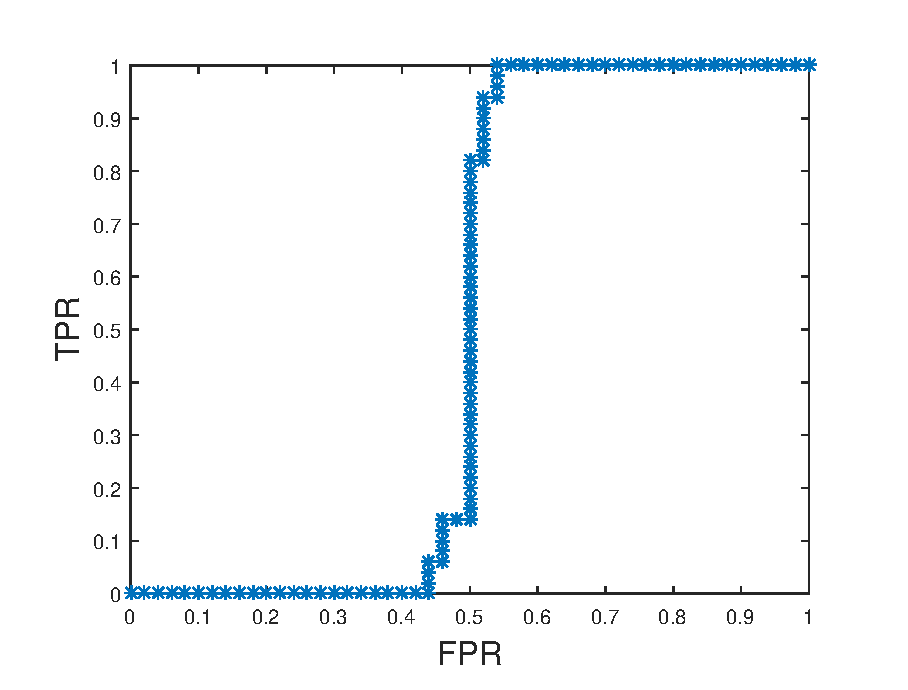
\includegraphics[width=0.6\textwidth]{figuras/prueba.eps}
	\caption{Pie de figura. Poner aquí cita del lugar de donde 
	se ha tomado la imagen en caso de que sea así. }
	\label{fig:prueba}
\end{figure}
\end{verbatim}

% Y ahora pongo la plantilla para que se incluya la figura efectivamente
\begin{figure}[t]
	\centering
	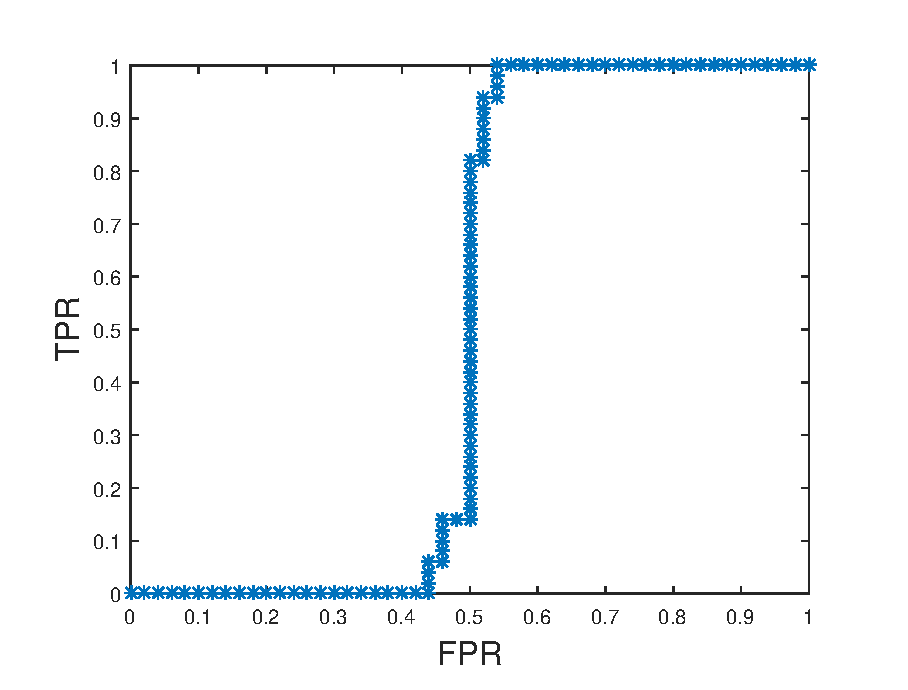
\includegraphics[width=0.6\textwidth]{figuras/prueba.eps}
	\caption{Pie de figura. Poner aquí cita del lugar de donde se ha tomado la imagen en caso de que sea así. }
	\label{fig:prueba}
\end{figure}

Si se pone el modificador [t] (top) latex ubicará la figura en la parte de arriba de la página. Ver otros modificadores como [h] (here) o [b] (bottom). Se pueden usar otras plantillas para, por ejemplo, poner dos figuras una al lado de otra. Consultar en Internet diferentes plantillas en caso de necesidad. 

Cuando en el texto nos refiramos a la figura en cuestión por el número, debemos usar la mayúscula y utilizar referencia a la figura. Esto hará que no nos tengamos que preocupar de la numeración de las figuras. Ej. Como se puede comprobar en la Figura~\ref{fig:prueba}.

Sustituir expresiones del tipo: “En la siguiente figura…” por “En la Figura 2.2…”


\subsection*{Inserción de tablas}

Este sería un ejemplo de una tabla. Se puede modificar el formato y contenido (ver en Internet algún enlace sobre cómo formatear tablas en latex). 

\begin{table}[t]
	\caption{Descripción de la tabla.}
	\label{table:prueba}
	\centering
	\begin{tabular}{l  c} 
		\hline \\[-1.5ex]
		\textbf{Tipo de ataque} & \textbf{Etiqueta} \\ [1ex] 
		\hline\hline \\[-1.5ex]
		DoS11 & dos \\ [0.5ex]
		Exf1MBp & exf1KB \\ [1ex]
		\hline
	\end{tabular}
\end{table}

La forma de referirse a las tablas es similar a las de las figuras (usar mayúsculas y referencia a la etiqueta(label) de la tabla). Ej. Como se puede ver en la Tabla~\ref{table:prueba}, ...


\subsection*{Citas de bibliografía}
Ejemplo de cita de bibliografía. Primero se va a google.scholar y se busca la referencia. Después se da al enlace citar, y se elige el formato bibtex. Se copia ese texto en el fichero bibliografia.bib. Un ejemplo de referenciar una cita es \cite{macia2008evaluation}.


\subsection*{Referencias a secciones}

Para referirnos a secciones, primero debemos tener una etiqueta de tipo \texttt{label} en dicha sección. Posteriormente, pondremos una referencia a dicho label, igual que hacemos para las figuras y las tablas. Ej. Como se ha mencionado en la Sección~\ref{sec:intro:motivacion} (Nótese que la palabra Sección va con mayúscula).

\subsection*{Glosario y acrónimos}

Cuando se utilice un acrónimo se debe definir en el fichero glosario/entradas\_glosario, tal y como está el ejemplo en dicho fichero. Al referirse en el texto se indicará así: \gls{svm} (ver que la primera vez lo pondrá completo). La segunda vez que se referencie a \gls{svm} ya no aparece completo. También se puede nombrar en plural así: \glspl{svm}. 
Otros ejemplos de acrónimo son: \gls{gcd}, \gls{lcm}, \gls{gmf}. 

A la hora de compilar con el glosario, se debe abrir una terminal CMD en el directorio de los fuentes latex del proyecto, y ejecutar el siguiente comando: \texttt{makeglossaries proyecto}. Esto generará los ficheros auxiliares que contienen el glosario. 

\subsection*{Listados de código}

Aquí se puede ver un ejemplo de listado de código: 

%\begin{lstlisting}[frame=none, numbers=none]


\begin{lstlisting}[language=Python,caption=Ejemplo de Python, label=listado:pythonPrueba]
import numpy as np

def incmatrix(genl1,genl2):
	m = len(genl1)
	n = len(genl2)
	M = None #to become the incidence matrix
	VT = np.zeros((n*m,1), int)  #dummy variable

	#compute the bitwise xor matrix
	M1 = bitxormatrix(genl1)
	M2 = np.triu(bitxormatrix(genl2),1) 
	
	for i in range(m-1):
		for j in range(i+1, m):
			[r,c] = np.where(M2 == M1[i,j])
			for k in range(len(r)):
				VT[(i)*n + r[k]] = 1;
				VT[(i)*n + c[k]] = 1;
				VT[(j)*n + r[k]] = 1;
				VT[(j)*n + c[k]] = 1;
	
	if M is None:
		M = np.copy(VT)
	else:
		M = np.concatenate((M, VT), 1)
	
	VT = np.zeros((n*m,1), int)
	
	return M

\end{lstlisting}

Nos podemos referir a él como Listado de código~\ref{listado:pythonPrueba}. 
Si queremos que aparezca como un flotante en la página debemos poner la palabra \texttt{float} así: 
\begin{verbatim}
\begin{lstlisting}[float,language=Python,caption=Ejemplo de Python, 
label=listado:pythonPrueba]
\end{verbatim}


\subsection*{Enlaces URL}
Podemos poner un enlace así \url{http://dtstc.ugr.es/~gmacia} --> %

\chapter*{Guía de estilo para escribir un TFG/TFM} \addcontentsline{toc}{chapter}{Guía de estilo}

Este capítulo no forma parte del TFG/TFM. Su único objetivo es aportar algunas recomendaciones y plantillas para tener claro cómo redactar el TFG/TFM. Una vez se haya comprendido, se puede comentar la siguiente línea en el fichero proyecto.tex añadiéndole al principio el carácter \%: 
\begin{verbatim}
\input{guiaDeEstilo} --> %\input{guiaDeEstilo}
\end{verbatim}

\section*{Recomendaciones generales}
A la hora de escribir el TFG/TFM es importante seguir las siguientes recomendaciones: 

\begin{enumerate}
	\item La memoria debe realizarse con el \textbf{máximo cuidado}, y debe proporcionar de forma consistente -y por sí misma- una idea clara y concisa de lo que se ha realizado. 
	\item No debe tener errores tipográficos ni ortográficos. Este es un aspecto que penaliza muchísimo el trabajo en la evaluación del tribunal. 
	\item Siempre que se utilice alguna figura no elaborada por el autor del proyecto debe indicarse la fuente de la que se ha sacado mediante una cita en la bibliografía. 
	\item La lectura debe ser fluida. Por ello, dada la dificultad que tiene afrontar la escritura de un texto largo casi por primera vez, se recomienda elaborar un índice rellenando los títulos de los diferentes apartados de que constará este documento. En segundo lugar, para cada apartado, se indicarán a modo de resumen las diferentes ideas que se desarrollarán posteriormente (una línea de texto por idea). Después, se desarrollan las ideas (cada idea en un párrafo). Cuando se termina, se realiza una lectura completa y detallada del texto para comprobar que es coherente y no tiene fallos ortográficos, tipográficos ni gramaticales, antes de pasarlo al tutor. 
	\item Una extensión normal está entorno a las 100-120 páginas. Esto no quiere decir que tengamos que escribir por escribir, ni meter contenido adicional sin sentido. Hay que escribir el proyecto de forma coherente, pero sin ser telegráfico, esto es, realizando una descripción detallada del trabajo realizado. 
	\item Evitar afirmaciones del tipo “El sistema diseñado es bastante bueno”. Esa misma frase debería ser escrita tal que responda a las preguntas: ¿Qué parte del sistema? ¿En qué sentido? ¿Cuánto de bueno? ¿Comparado con qué?
	\item Evitar la primera persona (incluso del plural). No obstante para resaltar la autoría de algo o enfatizar una posición personal sí se puede usar.
	\item Numerar estructuradamente los capítulos, secciones y subsecciones. Evitar más de tres niveles de anidamiento. 
	\item Toda afirmación categórica o se demuestra (teórica o experimentalmente)  o se incluye una referencia en la que se haya previamente demostrado.
	\item Toda tecnología, teorema, institución, norma, documento que se mencione debe estar referenciado. No incluir referencias a la wiki.
	\item Los términos en ingles que no tenga sentido traducir se pondrán en cursiva al menos para indicar que es un término no castellano.
	 

\end{enumerate}

\section*{Recomendaciones específicas para determinados contenidos}

\subsection*{Inserción de figuras}
Esta es una plantilla de código para adjuntar una figura. 

% El verbatim es solo para poner en el PDF el código que corresponde a la inserción de la figura
\begin{verbatim}
\begin{figure}[t]
	\centering
		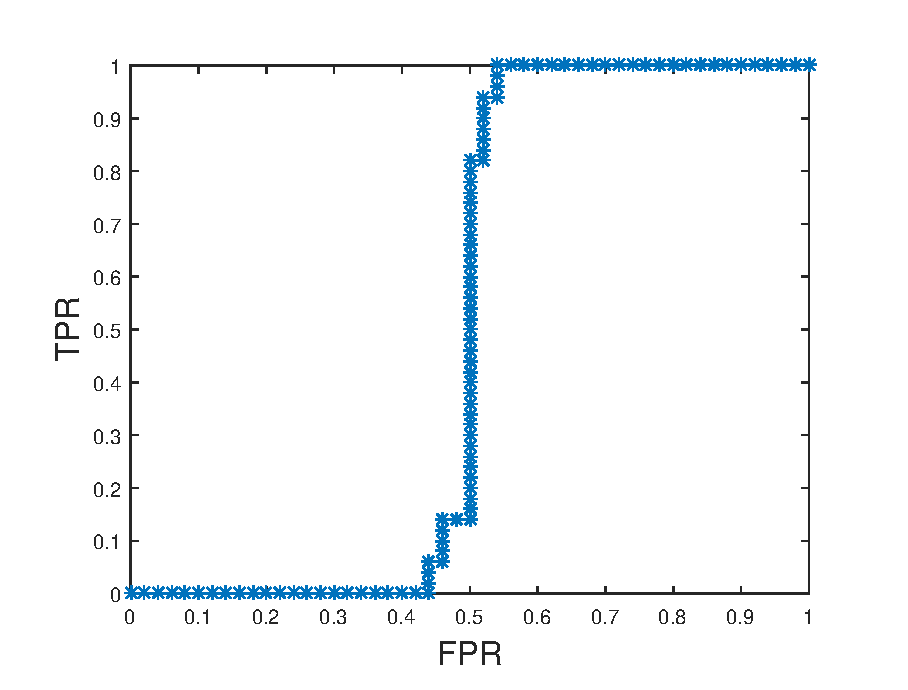
\includegraphics[width=0.6\textwidth]{figuras/prueba.eps}
	\caption{Pie de figura. Poner aquí cita del lugar de donde 
	se ha tomado la imagen en caso de que sea así. }
	\label{fig:prueba}
\end{figure}
\end{verbatim}

% Y ahora pongo la plantilla para que se incluya la figura efectivamente
\begin{figure}[t]
	\centering
	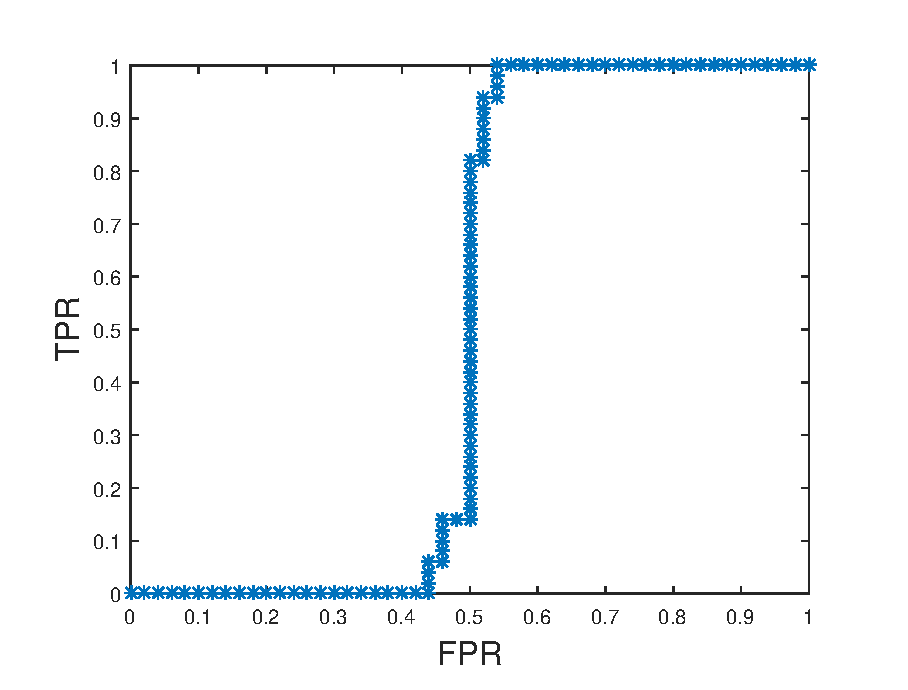
\includegraphics[width=0.6\textwidth]{figuras/prueba.eps}
	\caption{Pie de figura. Poner aquí cita del lugar de donde se ha tomado la imagen en caso de que sea así. }
	\label{fig:prueba}
\end{figure}

Si se pone el modificador [t] (top) latex ubicará la figura en la parte de arriba de la página. Ver otros modificadores como [h] (here) o [b] (bottom). Se pueden usar otras plantillas para, por ejemplo, poner dos figuras una al lado de otra. Consultar en Internet diferentes plantillas en caso de necesidad. 

Cuando en el texto nos refiramos a la figura en cuestión por el número, debemos usar la mayúscula y utilizar referencia a la figura. Esto hará que no nos tengamos que preocupar de la numeración de las figuras. Ej. Como se puede comprobar en la Figura~\ref{fig:prueba}.

Sustituir expresiones del tipo: “En la siguiente figura…” por “En la Figura 2.2…”


\subsection*{Inserción de tablas}

Este sería un ejemplo de una tabla. Se puede modificar el formato y contenido (ver en Internet algún enlace sobre cómo formatear tablas en latex). 

\begin{table}[t]
	\caption{Descripción de la tabla.}
	\label{table:prueba}
	\centering
	\begin{tabular}{l  c} 
		\hline \\[-1.5ex]
		\textbf{Tipo de ataque} & \textbf{Etiqueta} \\ [1ex] 
		\hline\hline \\[-1.5ex]
		DoS11 & dos \\ [0.5ex]
		Exf1MBp & exf1KB \\ [1ex]
		\hline
	\end{tabular}
\end{table}

La forma de referirse a las tablas es similar a las de las figuras (usar mayúsculas y referencia a la etiqueta(label) de la tabla). Ej. Como se puede ver en la Tabla~\ref{table:prueba}, ...


\subsection*{Citas de bibliografía}
Ejemplo de cita de bibliografía. Primero se va a google.scholar y se busca la referencia. Después se da al enlace citar, y se elige el formato bibtex. Se copia ese texto en el fichero bibliografia.bib. Un ejemplo de referenciar una cita es \cite{macia2008evaluation}.


\subsection*{Referencias a secciones}

Para referirnos a secciones, primero debemos tener una etiqueta de tipo \texttt{label} en dicha sección. Posteriormente, pondremos una referencia a dicho label, igual que hacemos para las figuras y las tablas. Ej. Como se ha mencionado en la Sección~\ref{sec:intro:motivacion} (Nótese que la palabra Sección va con mayúscula).

\subsection*{Glosario y acrónimos}

Cuando se utilice un acrónimo se debe definir en el fichero glosario/entradas\_glosario, tal y como está el ejemplo en dicho fichero. Al referirse en el texto se indicará así: \gls{svm} (ver que la primera vez lo pondrá completo). La segunda vez que se referencie a \gls{svm} ya no aparece completo. También se puede nombrar en plural así: \glspl{svm}. 
Otros ejemplos de acrónimo son: \gls{gcd}, \gls{lcm}, \gls{gmf}. 

A la hora de compilar con el glosario, se debe abrir una terminal CMD en el directorio de los fuentes latex del proyecto, y ejecutar el siguiente comando: \texttt{makeglossaries proyecto}. Esto generará los ficheros auxiliares que contienen el glosario. 

\subsection*{Listados de código}

Aquí se puede ver un ejemplo de listado de código: 

%\begin{lstlisting}[frame=none, numbers=none]


\begin{lstlisting}[language=Python,caption=Ejemplo de Python, label=listado:pythonPrueba]
import numpy as np

def incmatrix(genl1,genl2):
	m = len(genl1)
	n = len(genl2)
	M = None #to become the incidence matrix
	VT = np.zeros((n*m,1), int)  #dummy variable

	#compute the bitwise xor matrix
	M1 = bitxormatrix(genl1)
	M2 = np.triu(bitxormatrix(genl2),1) 
	
	for i in range(m-1):
		for j in range(i+1, m):
			[r,c] = np.where(M2 == M1[i,j])
			for k in range(len(r)):
				VT[(i)*n + r[k]] = 1;
				VT[(i)*n + c[k]] = 1;
				VT[(j)*n + r[k]] = 1;
				VT[(j)*n + c[k]] = 1;
	
	if M is None:
		M = np.copy(VT)
	else:
		M = np.concatenate((M, VT), 1)
	
	VT = np.zeros((n*m,1), int)
	
	return M

\end{lstlisting}

Nos podemos referir a él como Listado de código~\ref{listado:pythonPrueba}. 
Si queremos que aparezca como un flotante en la página debemos poner la palabra \texttt{float} así: 
\begin{verbatim}
\begin{lstlisting}[float,language=Python,caption=Ejemplo de Python, 
label=listado:pythonPrueba]
\end{verbatim}


\subsection*{Enlaces URL}
Podemos poner un enlace así \url{http://dtstc.ugr.es/~gmacia}
\end{verbatim}

\section*{Recomendaciones generales}
A la hora de escribir el TFG/TFM es importante seguir las siguientes recomendaciones: 

\begin{enumerate}
	\item La memoria debe realizarse con el \textbf{máximo cuidado}, y debe proporcionar de forma consistente -y por sí misma- una idea clara y concisa de lo que se ha realizado. 
	\item No debe tener errores tipográficos ni ortográficos. Este es un aspecto que penaliza muchísimo el trabajo en la evaluación del tribunal. 
	\item Siempre que se utilice alguna figura no elaborada por el autor del proyecto debe indicarse la fuente de la que se ha sacado mediante una cita en la bibliografía. 
	\item La lectura debe ser fluida. Por ello, dada la dificultad que tiene afrontar la escritura de un texto largo casi por primera vez, se recomienda elaborar un índice rellenando los títulos de los diferentes apartados de que constará este documento. En segundo lugar, para cada apartado, se indicarán a modo de resumen las diferentes ideas que se desarrollarán posteriormente (una línea de texto por idea). Después, se desarrollan las ideas (cada idea en un párrafo). Cuando se termina, se realiza una lectura completa y detallada del texto para comprobar que es coherente y no tiene fallos ortográficos, tipográficos ni gramaticales, antes de pasarlo al tutor. 
	\item Una extensión normal está entorno a las 100-120 páginas. Esto no quiere decir que tengamos que escribir por escribir, ni meter contenido adicional sin sentido. Hay que escribir el proyecto de forma coherente, pero sin ser telegráfico, esto es, realizando una descripción detallada del trabajo realizado. 
	\item Evitar afirmaciones del tipo “El sistema diseñado es bastante bueno”. Esa misma frase debería ser escrita tal que responda a las preguntas: ¿Qué parte del sistema? ¿En qué sentido? ¿Cuánto de bueno? ¿Comparado con qué?
	\item Evitar la primera persona (incluso del plural). No obstante para resaltar la autoría de algo o enfatizar una posición personal sí se puede usar.
	\item Numerar estructuradamente los capítulos, secciones y subsecciones. Evitar más de tres niveles de anidamiento. 
	\item Toda afirmación categórica o se demuestra (teórica o experimentalmente)  o se incluye una referencia en la que se haya previamente demostrado.
	\item Toda tecnología, teorema, institución, norma, documento que se mencione debe estar referenciado. No incluir referencias a la wiki.
	\item Los términos en ingles que no tenga sentido traducir se pondrán en cursiva al menos para indicar que es un término no castellano.
	 

\end{enumerate}

\section*{Recomendaciones específicas para determinados contenidos}

\subsection*{Inserción de figuras}
Esta es una plantilla de código para adjuntar una figura. 

% El verbatim es solo para poner en el PDF el código que corresponde a la inserción de la figura
\begin{verbatim}
\begin{figure}[t]
	\centering
		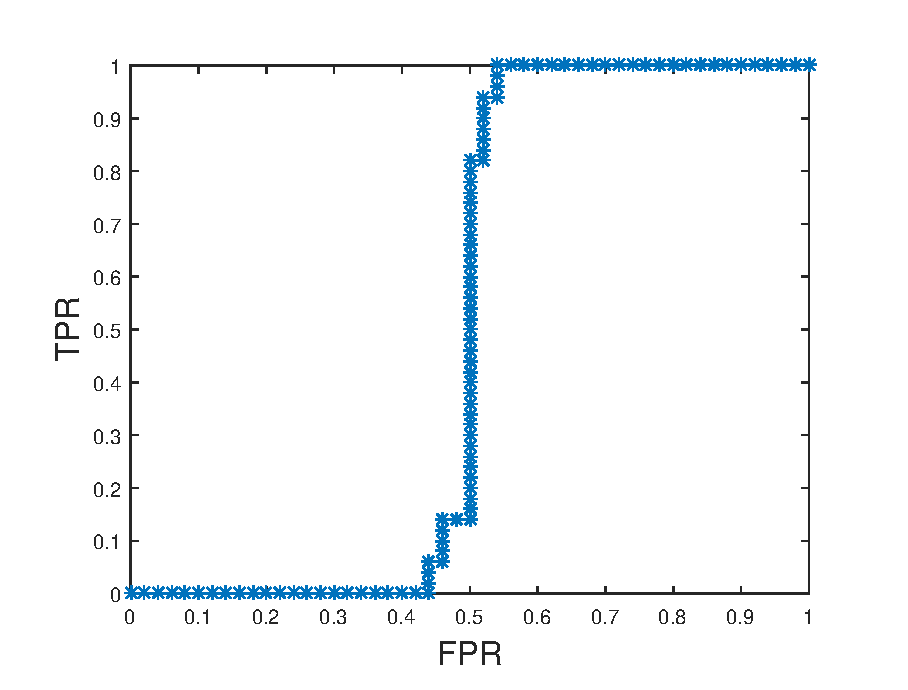
\includegraphics[width=0.6\textwidth]{figuras/prueba.eps}
	\caption{Pie de figura. Poner aquí cita del lugar de donde 
	se ha tomado la imagen en caso de que sea así. }
	\label{fig:prueba}
\end{figure}
\end{verbatim}

% Y ahora pongo la plantilla para que se incluya la figura efectivamente
\begin{figure}[t]
	\centering
	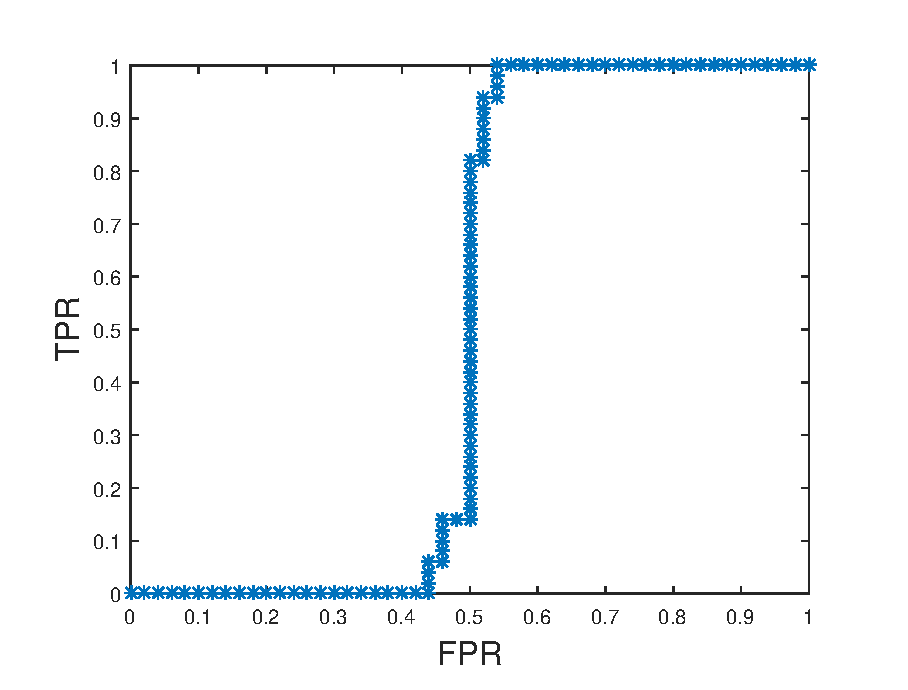
\includegraphics[width=0.6\textwidth]{figuras/prueba.eps}
	\caption{Pie de figura. Poner aquí cita del lugar de donde se ha tomado la imagen en caso de que sea así. }
	\label{fig:prueba}
\end{figure}

Si se pone el modificador [t] (top) latex ubicará la figura en la parte de arriba de la página. Ver otros modificadores como [h] (here) o [b] (bottom). Se pueden usar otras plantillas para, por ejemplo, poner dos figuras una al lado de otra. Consultar en Internet diferentes plantillas en caso de necesidad. 

Cuando en el texto nos refiramos a la figura en cuestión por el número, debemos usar la mayúscula y utilizar referencia a la figura. Esto hará que no nos tengamos que preocupar de la numeración de las figuras. Ej. Como se puede comprobar en la Figura~\ref{fig:prueba}.

Sustituir expresiones del tipo: “En la siguiente figura…” por “En la Figura 2.2…”


\subsection*{Inserción de tablas}

Este sería un ejemplo de una tabla. Se puede modificar el formato y contenido (ver en Internet algún enlace sobre cómo formatear tablas en latex). 

\begin{table}[t]
	\caption{Descripción de la tabla.}
	\label{table:prueba}
	\centering
	\begin{tabular}{l  c} 
		\hline \\[-1.5ex]
		\textbf{Tipo de ataque} & \textbf{Etiqueta} \\ [1ex] 
		\hline\hline \\[-1.5ex]
		DoS11 & dos \\ [0.5ex]
		Exf1MBp & exf1KB \\ [1ex]
		\hline
	\end{tabular}
\end{table}

La forma de referirse a las tablas es similar a las de las figuras (usar mayúsculas y referencia a la etiqueta(label) de la tabla). Ej. Como se puede ver en la Tabla~\ref{table:prueba}, ...


\subsection*{Citas de bibliografía}
Ejemplo de cita de bibliografía. Primero se va a google.scholar y se busca la referencia. Después se da al enlace citar, y se elige el formato bibtex. Se copia ese texto en el fichero bibliografia.bib. Un ejemplo de referenciar una cita es \cite{macia2008evaluation}.


\subsection*{Referencias a secciones}

Para referirnos a secciones, primero debemos tener una etiqueta de tipo \texttt{label} en dicha sección. Posteriormente, pondremos una referencia a dicho label, igual que hacemos para las figuras y las tablas. Ej. Como se ha mencionado en la Sección~\ref{sec:intro:motivacion} (Nótese que la palabra Sección va con mayúscula).

\subsection*{Glosario y acrónimos}

Cuando se utilice un acrónimo se debe definir en el fichero glosario/entradas\_glosario, tal y como está el ejemplo en dicho fichero. Al referirse en el texto se indicará así: \gls{svm} (ver que la primera vez lo pondrá completo). La segunda vez que se referencie a \gls{svm} ya no aparece completo. También se puede nombrar en plural así: \glspl{svm}. 
Otros ejemplos de acrónimo son: \gls{gcd}, \gls{lcm}, \gls{gmf}. 

A la hora de compilar con el glosario, se debe abrir una terminal CMD en el directorio de los fuentes latex del proyecto, y ejecutar el siguiente comando: \texttt{makeglossaries proyecto}. Esto generará los ficheros auxiliares que contienen el glosario. 

\subsection*{Listados de código}

Aquí se puede ver un ejemplo de listado de código: 

%\begin{lstlisting}[frame=none, numbers=none]


\begin{lstlisting}[language=Python,caption=Ejemplo de Python, label=listado:pythonPrueba]
import numpy as np

def incmatrix(genl1,genl2):
	m = len(genl1)
	n = len(genl2)
	M = None #to become the incidence matrix
	VT = np.zeros((n*m,1), int)  #dummy variable

	#compute the bitwise xor matrix
	M1 = bitxormatrix(genl1)
	M2 = np.triu(bitxormatrix(genl2),1) 
	
	for i in range(m-1):
		for j in range(i+1, m):
			[r,c] = np.where(M2 == M1[i,j])
			for k in range(len(r)):
				VT[(i)*n + r[k]] = 1;
				VT[(i)*n + c[k]] = 1;
				VT[(j)*n + r[k]] = 1;
				VT[(j)*n + c[k]] = 1;
	
	if M is None:
		M = np.copy(VT)
	else:
		M = np.concatenate((M, VT), 1)
	
	VT = np.zeros((n*m,1), int)
	
	return M

\end{lstlisting}

Nos podemos referir a él como Listado de código~\ref{listado:pythonPrueba}. 
Si queremos que aparezca como un flotante en la página debemos poner la palabra \texttt{float} así: 
\begin{verbatim}
\begin{lstlisting}[float,language=Python,caption=Ejemplo de Python, 
label=listado:pythonPrueba]
\end{verbatim}


\subsection*{Enlaces URL}
Podemos poner un enlace así \url{http://dtstc.ugr.es/~gmacia}
\end{verbatim}

\section*{Recomendaciones generales}
A la hora de escribir el TFG/TFM es importante seguir las siguientes recomendaciones: 

\begin{enumerate}
	\item La memoria debe realizarse con el \textbf{máximo cuidado}, y debe proporcionar de forma consistente -y por sí misma- una idea clara y concisa de lo que se ha realizado. 
	\item No debe tener errores tipográficos ni ortográficos. Este es un aspecto que penaliza muchísimo el trabajo en la evaluación del tribunal. 
	\item Siempre que se utilice alguna figura no elaborada por el autor del proyecto debe indicarse la fuente de la que se ha sacado mediante una cita en la bibliografía. 
	\item La lectura debe ser fluida. Por ello, dada la dificultad que tiene afrontar la escritura de un texto largo casi por primera vez, se recomienda elaborar un índice rellenando los títulos de los diferentes apartados de que constará este documento. En segundo lugar, para cada apartado, se indicarán a modo de resumen las diferentes ideas que se desarrollarán posteriormente (una línea de texto por idea). Después, se desarrollan las ideas (cada idea en un párrafo). Cuando se termina, se realiza una lectura completa y detallada del texto para comprobar que es coherente y no tiene fallos ortográficos, tipográficos ni gramaticales, antes de pasarlo al tutor. 
	\item Una extensión normal está entorno a las 100-120 páginas. Esto no quiere decir que tengamos que escribir por escribir, ni meter contenido adicional sin sentido. Hay que escribir el proyecto de forma coherente, pero sin ser telegráfico, esto es, realizando una descripción detallada del trabajo realizado. 
	\item Evitar afirmaciones del tipo “El sistema diseñado es bastante bueno”. Esa misma frase debería ser escrita tal que responda a las preguntas: ¿Qué parte del sistema? ¿En qué sentido? ¿Cuánto de bueno? ¿Comparado con qué?
	\item Evitar la primera persona (incluso del plural). No obstante para resaltar la autoría de algo o enfatizar una posición personal sí se puede usar.
	\item Numerar estructuradamente los capítulos, secciones y subsecciones. Evitar más de tres niveles de anidamiento. 
	\item Toda afirmación categórica o se demuestra (teórica o experimentalmente)  o se incluye una referencia en la que se haya previamente demostrado.
	\item Toda tecnología, teorema, institución, norma, documento que se mencione debe estar referenciado. No incluir referencias a la wiki.
	\item Los términos en ingles que no tenga sentido traducir se pondrán en cursiva al menos para indicar que es un término no castellano.
	 

\end{enumerate}

\section*{Recomendaciones específicas para determinados contenidos}

\subsection*{Inserción de figuras}
Esta es una plantilla de código para adjuntar una figura. 

% El verbatim es solo para poner en el PDF el código que corresponde a la inserción de la figura
\begin{verbatim}
\begin{figure}[t]
	\centering
		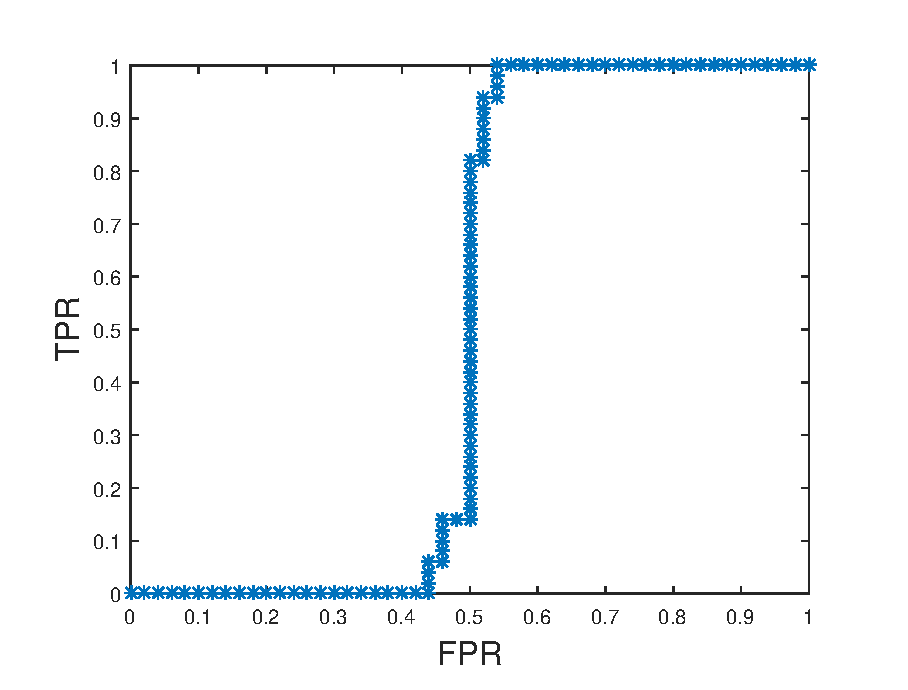
\includegraphics[width=0.6\textwidth]{figuras/prueba.eps}
	\caption{Pie de figura. Poner aquí cita del lugar de donde 
	se ha tomado la imagen en caso de que sea así. }
	\label{fig:prueba}
\end{figure}
\end{verbatim}

% Y ahora pongo la plantilla para que se incluya la figura efectivamente
\begin{figure}[t]
	\centering
	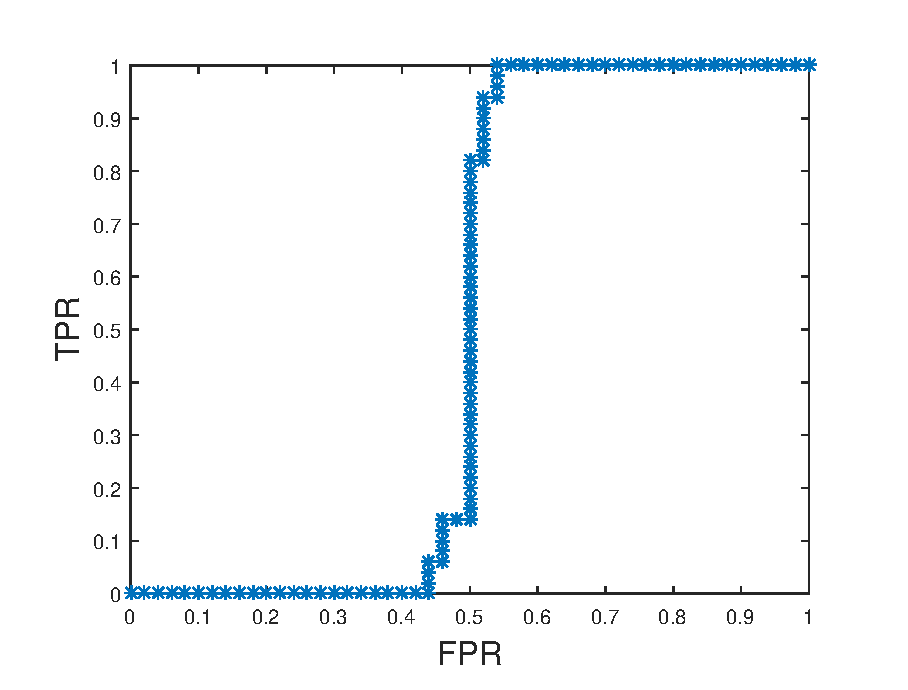
\includegraphics[width=0.6\textwidth]{figuras/prueba.eps}
	\caption{Pie de figura. Poner aquí cita del lugar de donde se ha tomado la imagen en caso de que sea así. }
	\label{fig:prueba}
\end{figure}

Si se pone el modificador [t] (top) latex ubicará la figura en la parte de arriba de la página. Ver otros modificadores como [h] (here) o [b] (bottom). Se pueden usar otras plantillas para, por ejemplo, poner dos figuras una al lado de otra. Consultar en Internet diferentes plantillas en caso de necesidad. 

Cuando en el texto nos refiramos a la figura en cuestión por el número, debemos usar la mayúscula y utilizar referencia a la figura. Esto hará que no nos tengamos que preocupar de la numeración de las figuras. Ej. Como se puede comprobar en la Figura~\ref{fig:prueba}.

Sustituir expresiones del tipo: “En la siguiente figura…” por “En la Figura 2.2…”


\subsection*{Inserción de tablas}

Este sería un ejemplo de una tabla. Se puede modificar el formato y contenido (ver en Internet algún enlace sobre cómo formatear tablas en latex). 

\begin{table}[t]
	\caption{Descripción de la tabla.}
	\label{table:prueba}
	\centering
	\begin{tabular}{l  c} 
		\hline \\[-1.5ex]
		\textbf{Tipo de ataque} & \textbf{Etiqueta} \\ [1ex] 
		\hline\hline \\[-1.5ex]
		DoS11 & dos \\ [0.5ex]
		Exf1MBp & exf1KB \\ [1ex]
		\hline
	\end{tabular}
\end{table}

La forma de referirse a las tablas es similar a las de las figuras (usar mayúsculas y referencia a la etiqueta(label) de la tabla). Ej. Como se puede ver en la Tabla~\ref{table:prueba}, ...


\subsection*{Citas de bibliografía}
Ejemplo de cita de bibliografía. Primero se va a google.scholar y se busca la referencia. Después se da al enlace citar, y se elige el formato bibtex. Se copia ese texto en el fichero bibliografia.bib. Un ejemplo de referenciar una cita es \cite{macia2008evaluation}.


\subsection*{Referencias a secciones}

Para referirnos a secciones, primero debemos tener una etiqueta de tipo \texttt{label} en dicha sección. Posteriormente, pondremos una referencia a dicho label, igual que hacemos para las figuras y las tablas. Ej. Como se ha mencionado en la Sección~\ref{sec:intro:motivacion} (Nótese que la palabra Sección va con mayúscula).

\subsection*{Glosario y acrónimos}

Cuando se utilice un acrónimo se debe definir en el fichero glosario/entradas\_glosario, tal y como está el ejemplo en dicho fichero. Al referirse en el texto se indicará así: \gls{svm} (ver que la primera vez lo pondrá completo). La segunda vez que se referencie a \gls{svm} ya no aparece completo. También se puede nombrar en plural así: \glspl{svm}. 
Otros ejemplos de acrónimo son: \gls{gcd}, \gls{lcm}, \gls{gmf}. 

A la hora de compilar con el glosario, se debe abrir una terminal CMD en el directorio de los fuentes latex del proyecto, y ejecutar el siguiente comando: \texttt{makeglossaries proyecto}. Esto generará los ficheros auxiliares que contienen el glosario. 

\subsection*{Listados de código}

Aquí se puede ver un ejemplo de listado de código: 

%\begin{lstlisting}[frame=none, numbers=none]


\begin{lstlisting}[language=Python,caption=Ejemplo de Python, label=listado:pythonPrueba]
import numpy as np

def incmatrix(genl1,genl2):
	m = len(genl1)
	n = len(genl2)
	M = None #to become the incidence matrix
	VT = np.zeros((n*m,1), int)  #dummy variable

	#compute the bitwise xor matrix
	M1 = bitxormatrix(genl1)
	M2 = np.triu(bitxormatrix(genl2),1) 
	
	for i in range(m-1):
		for j in range(i+1, m):
			[r,c] = np.where(M2 == M1[i,j])
			for k in range(len(r)):
				VT[(i)*n + r[k]] = 1;
				VT[(i)*n + c[k]] = 1;
				VT[(j)*n + r[k]] = 1;
				VT[(j)*n + c[k]] = 1;
	
	if M is None:
		M = np.copy(VT)
	else:
		M = np.concatenate((M, VT), 1)
	
	VT = np.zeros((n*m,1), int)
	
	return M

\end{lstlisting}

Nos podemos referir a él como Listado de código~\ref{listado:pythonPrueba}. 
Si queremos que aparezca como un flotante en la página debemos poner la palabra \texttt{float} así: 
\begin{verbatim}
\begin{lstlisting}[float,language=Python,caption=Ejemplo de Python, 
label=listado:pythonPrueba]
\end{verbatim}


\subsection*{Enlaces URL}
Podemos poner un enlace así \url{http://dtstc.ugr.es/~gmacia}
\end{verbatim}

\section*{Recomendaciones generales}
A la hora de escribir el TFG/TFM es importante seguir las siguientes recomendaciones: 

\begin{enumerate}
	\item La memoria debe realizarse con el \textbf{máximo cuidado}, y debe proporcionar de forma consistente -y por sí misma- una idea clara y concisa de lo que se ha realizado. 
	\item No debe tener errores tipográficos ni ortográficos. Este es un aspecto que penaliza muchísimo el trabajo en la evaluación del tribunal. 
	\item Siempre que se utilice alguna figura no elaborada por el autor del proyecto debe indicarse la fuente de la que se ha sacado mediante una cita en la bibliografía. 
	\item La lectura debe ser fluida. Por ello, dada la dificultad que tiene afrontar la escritura de un texto largo casi por primera vez, se recomienda elaborar un índice rellenando los títulos de los diferentes apartados de que constará este documento. En segundo lugar, para cada apartado, se indicarán a modo de resumen las diferentes ideas que se desarrollarán posteriormente (una línea de texto por idea). Después, se desarrollan las ideas (cada idea en un párrafo). Cuando se termina, se realiza una lectura completa y detallada del texto para comprobar que es coherente y no tiene fallos ortográficos, tipográficos ni gramaticales, antes de pasarlo al tutor. 
	\item Una extensión normal está entorno a las 100-120 páginas. Esto no quiere decir que tengamos que escribir por escribir, ni meter contenido adicional sin sentido. Hay que escribir el proyecto de forma coherente, pero sin ser telegráfico, esto es, realizando una descripción detallada del trabajo realizado. 
	\item Evitar afirmaciones del tipo “El sistema diseñado es bastante bueno”. Esa misma frase debería ser escrita tal que responda a las preguntas: ¿Qué parte del sistema? ¿En qué sentido? ¿Cuánto de bueno? ¿Comparado con qué?
	\item Evitar la primera persona (incluso del plural). No obstante para resaltar la autoría de algo o enfatizar una posición personal sí se puede usar.
	\item Numerar estructuradamente los capítulos, secciones y subsecciones. Evitar más de tres niveles de anidamiento. 
	\item Toda afirmación categórica o se demuestra (teórica o experimentalmente)  o se incluye una referencia en la que se haya previamente demostrado.
	\item Toda tecnología, teorema, institución, norma, documento que se mencione debe estar referenciado. No incluir referencias a la wiki.
	\item Los términos en ingles que no tenga sentido traducir se pondrán en cursiva al menos para indicar que es un término no castellano.
	 

\end{enumerate}

\section*{Recomendaciones específicas para determinados contenidos}

\subsection*{Inserción de figuras}
Esta es una plantilla de código para adjuntar una figura. 

% El verbatim es solo para poner en el PDF el código que corresponde a la inserción de la figura
\begin{verbatim}
\begin{figure}[t]
	\centering
		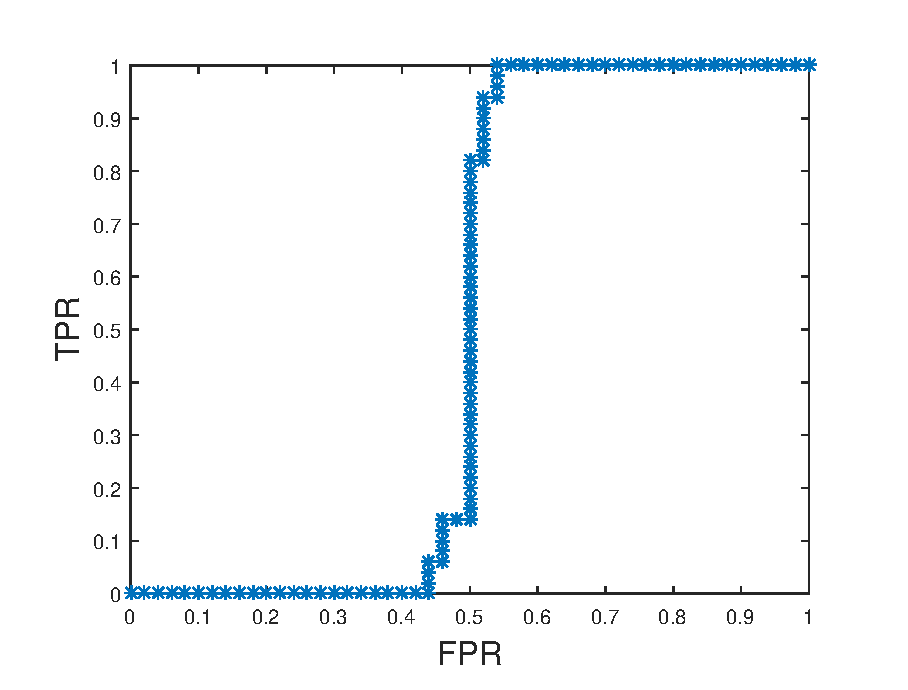
\includegraphics[width=0.6\textwidth]{figuras/prueba.eps}
	\caption{Pie de figura. Poner aquí cita del lugar de donde 
	se ha tomado la imagen en caso de que sea así. }
	\label{fig:prueba}
\end{figure}
\end{verbatim}

% Y ahora pongo la plantilla para que se incluya la figura efectivamente
\begin{figure}[t]
	\centering
	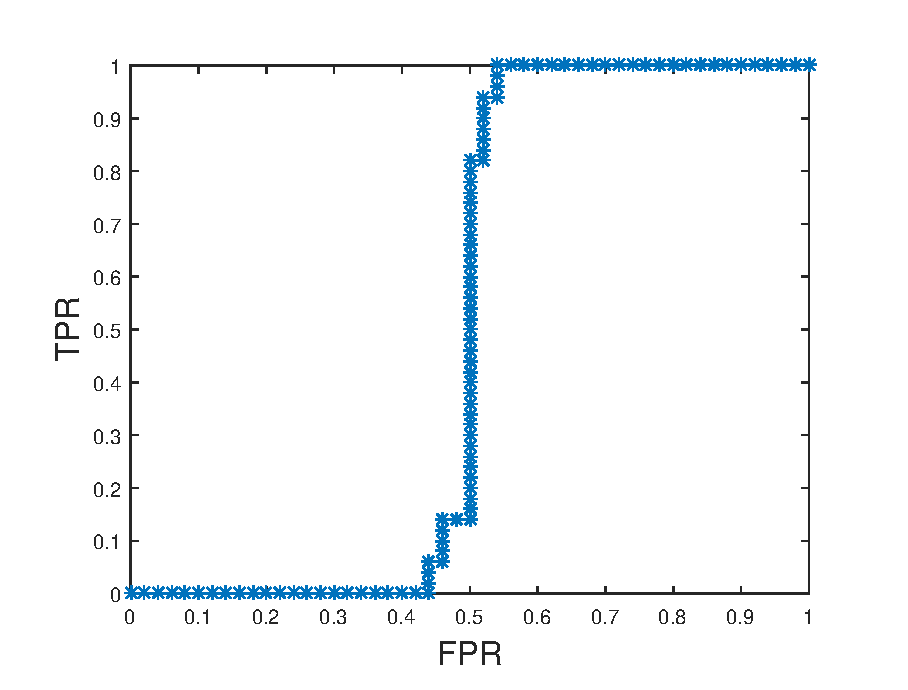
\includegraphics[width=0.6\textwidth]{figuras/prueba.eps}
	\caption{Pie de figura. Poner aquí cita del lugar de donde se ha tomado la imagen en caso de que sea así. }
	\label{fig:prueba}
\end{figure}

Si se pone el modificador [t] (top) latex ubicará la figura en la parte de arriba de la página. Ver otros modificadores como [h] (here) o [b] (bottom). Se pueden usar otras plantillas para, por ejemplo, poner dos figuras una al lado de otra. Consultar en Internet diferentes plantillas en caso de necesidad. 

Cuando en el texto nos refiramos a la figura en cuestión por el número, debemos usar la mayúscula y utilizar referencia a la figura. Esto hará que no nos tengamos que preocupar de la numeración de las figuras. Ej. Como se puede comprobar en la Figura~\ref{fig:prueba}.

Sustituir expresiones del tipo: “En la siguiente figura…” por “En la Figura 2.2…”


\subsection*{Inserción de tablas}

Este sería un ejemplo de una tabla. Se puede modificar el formato y contenido (ver en Internet algún enlace sobre cómo formatear tablas en latex). 

\begin{table}[t]
	\caption{Descripción de la tabla.}
	\label{table:prueba}
	\centering
	\begin{tabular}{l  c} 
		\hline \\[-1.5ex]
		\textbf{Tipo de ataque} & \textbf{Etiqueta} \\ [1ex] 
		\hline\hline \\[-1.5ex]
		DoS11 & dos \\ [0.5ex]
		Exf1MBp & exf1KB \\ [1ex]
		\hline
	\end{tabular}
\end{table}

La forma de referirse a las tablas es similar a las de las figuras (usar mayúsculas y referencia a la etiqueta(label) de la tabla). Ej. Como se puede ver en la Tabla~\ref{table:prueba}, ...


\subsection*{Citas de bibliografía}
Ejemplo de cita de bibliografía. Primero se va a google.scholar y se busca la referencia. Después se da al enlace citar, y se elige el formato bibtex. Se copia ese texto en el fichero bibliografia.bib. Un ejemplo de referenciar una cita es \cite{macia2008evaluation}.


\subsection*{Referencias a secciones}

Para referirnos a secciones, primero debemos tener una etiqueta de tipo \texttt{label} en dicha sección. Posteriormente, pondremos una referencia a dicho label, igual que hacemos para las figuras y las tablas. Ej. Como se ha mencionado en la Sección~\ref{sec:intro:motivacion} (Nótese que la palabra Sección va con mayúscula).

\subsection*{Glosario y acrónimos}

Cuando se utilice un acrónimo se debe definir en el fichero glosario/entradas\_glosario, tal y como está el ejemplo en dicho fichero. Al referirse en el texto se indicará así: \gls{svm} (ver que la primera vez lo pondrá completo). La segunda vez que se referencie a \gls{svm} ya no aparece completo. También se puede nombrar en plural así: \glspl{svm}. 
Otros ejemplos de acrónimo son: \gls{gcd}, \gls{lcm}, \gls{gmf}. 

A la hora de compilar con el glosario, se debe abrir una terminal CMD en el directorio de los fuentes latex del proyecto, y ejecutar el siguiente comando: \texttt{makeglossaries proyecto}. Esto generará los ficheros auxiliares que contienen el glosario. 

\subsection*{Listados de código}

Aquí se puede ver un ejemplo de listado de código: 

%\begin{lstlisting}[frame=none, numbers=none]


\begin{lstlisting}[language=Python,caption=Ejemplo de Python, label=listado:pythonPrueba]
import numpy as np

def incmatrix(genl1,genl2):
	m = len(genl1)
	n = len(genl2)
	M = None #to become the incidence matrix
	VT = np.zeros((n*m,1), int)  #dummy variable

	#compute the bitwise xor matrix
	M1 = bitxormatrix(genl1)
	M2 = np.triu(bitxormatrix(genl2),1) 
	
	for i in range(m-1):
		for j in range(i+1, m):
			[r,c] = np.where(M2 == M1[i,j])
			for k in range(len(r)):
				VT[(i)*n + r[k]] = 1;
				VT[(i)*n + c[k]] = 1;
				VT[(j)*n + r[k]] = 1;
				VT[(j)*n + c[k]] = 1;
	
	if M is None:
		M = np.copy(VT)
	else:
		M = np.concatenate((M, VT), 1)
	
	VT = np.zeros((n*m,1), int)
	
	return M

\end{lstlisting}

Nos podemos referir a él como Listado de código~\ref{listado:pythonPrueba}. 
Si queremos que aparezca como un flotante en la página debemos poner la palabra \texttt{float} así: 
\begin{verbatim}
\begin{lstlisting}[float,language=Python,caption=Ejemplo de Python, 
label=listado:pythonPrueba]
\end{verbatim}


\subsection*{Enlaces URL}
Podemos poner un enlace así \url{http://dtstc.ugr.es/~gmacia}